% From Bed Rest to Mars - written report, initial draft.
%
% Build (from this directory):
%   python ../report/make_figures.py      % or, from the repository root: python report/make_figures.py
%   pdflatex main && bibtex main && pdflatex main && pdflatex main
%
% Every table under generated/ and every figure under figures/ is written by make_figures.py
% from results/ and the frozen dataset. Numbers quoted in the prose were checked against the
% same files; if a result is refitted, rerun the script and re-read the prose against it.

\documentclass[11pt,a4paper]{article}

% --- encoding and fonts -------------------------------------------------------------------
\usepackage[T1]{fontenc}
\usepackage[utf8]{inputenc}
\usepackage{newtxtext}
\usepackage[varqu,varl]{inconsolata}
\usepackage{newtxmath}
\usepackage[final]{microtype}

% --- page -----------------------------------------------------------------------------------
\usepackage[a4paper,top=2.6cm,bottom=2.6cm,left=2.5cm,right=2.5cm,headheight=14pt]{geometry}
\linespread{1.06}
\setlength{\parskip}{0.35em}
\setlength{\parindent}{0pt}
\usepackage[dvipsnames]{xcolor}
\definecolor{accent}{HTML}{1C5CAB}
\definecolor{inktwo}{HTML}{52514E}
\definecolor{rulegrey}{HTML}{C3C2B7}
\definecolor{notebg}{HTML}{F4F7FC}

% --- structure ------------------------------------------------------------------------------
\usepackage{titlesec}
\titleformat{\section}{\sffamily\Large\bfseries\color{accent}}{\thesection}{0.8em}{}
\titleformat{\subsection}{\sffamily\large\bfseries}{\thesubsection}{0.7em}{}
\titleformat{\subsubsection}{\sffamily\normalsize\bfseries}{\thesubsubsection}{0.6em}{}
\titleformat{\paragraph}[runin]{\sffamily\normalsize\bfseries}{}{}{}[.]
\titlespacing*{\section}{0pt}{1.6em}{0.7em}
\titlespacing*{\subsection}{0pt}{1.2em}{0.45em}
\titlespacing*{\subsubsection}{0pt}{1.0em}{0.35em}
\titlespacing*{\paragraph}{0pt}{0.6em}{0.6em}
\setcounter{secnumdepth}{3}
\setcounter{tocdepth}{2}

\usepackage{fancyhdr}
\pagestyle{fancy}
\fancyhf{}
\fancyhead[L]{\sffamily\footnotesize\color{inktwo}From Bed Rest to Mars}
\fancyhead[R]{\sffamily\footnotesize\color{inktwo}Written report --- initial draft}
\fancyfoot[C]{\sffamily\footnotesize\thepage}
\renewcommand{\headrulewidth}{0.4pt}
\renewcommand{\headrule}{{\color{rulegrey}\hrule height \headrulewidth width \headwidth \vskip-\headrulewidth}}
\fancypagestyle{plain}{\fancyhf{}\fancyfoot[C]{\sffamily\footnotesize\thepage}\renewcommand{\headrulewidth}{0pt}}

% --- tables, figures, lists -----------------------------------------------------------------
\usepackage{graphicx}
\graphicspath{{figures/}}
\usepackage{booktabs}
\usepackage{tabularx}
\usepackage{longtable}
\usepackage{threeparttable}
\usepackage{makecell}
\usepackage{multirow}
\usepackage{array}
\usepackage{ragged2e}
\newcolumntype{L}[1]{>{\RaggedRight\arraybackslash}p{#1}}
\newcolumntype{Y}{>{\RaggedRight\arraybackslash}X}
\newcolumntype{P}[1]{>{\raggedright\arraybackslash}p{#1}}
\renewcommand{\arraystretch}{1.15}
\setlength{\tabcolsep}{5pt}
\usepackage[font=small,labelfont={bf,sf},labelsep=period,justification=justified,singlelinecheck=false,skip=6pt]{caption}
\captionsetup[table]{position=top}
\usepackage{subcaption}
\usepackage{float}
% Let text share pages with floats instead of leaving half-empty float pages.
\renewcommand{\topfraction}{0.9}
\renewcommand{\bottomfraction}{0.8}
\renewcommand{\textfraction}{0.07}
\renewcommand{\floatpagefraction}{0.85}
\setcounter{topnumber}{3}
\setcounter{bottomnumber}{2}
\setcounter{totalnumber}{5}
\usepackage{enumitem}
\setlist{itemsep=0.15em,topsep=0.3em,parsep=0.1em,leftmargin=1.6em}
\usepackage{amsmath}
\usepackage{bm}
\usepackage{siunitx}
\sisetup{detect-all,group-separator={,},group-minimum-digits=4}

% --- diagrams -------------------------------------------------------------------------------
\usepackage{tikz}
\usetikzlibrary{positioning,arrows.meta,calc,fit,backgrounds,shapes.misc}
\tikzset{
  box/.style={draw=rulegrey,rounded corners=2pt,fill=white,align=center,font=\sffamily\footnotesize,
              inner sep=4pt,text width=#1},
  box/.default=4.2cm,
  keybox/.style={box=#1,draw=accent,fill=notebg,line width=0.6pt},
  keybox/.default=4.2cm,
  sidebox/.style={draw=rulegrey,rounded corners=2pt,fill=gray!4,align=left,font=\sffamily\scriptsize,
                  inner sep=4pt,text width=#1},
  sidebox/.default=4.6cm,
  flow/.style={-{Stealth[length=5pt]},draw=inktwo,line width=0.6pt},
  stage/.style={font=\sffamily\scriptsize\bfseries,text=accent,rotate=90,anchor=south},
}

% --- references and links -------------------------------------------------------------------
\usepackage[numbers,sort&compress]{natbib}
\setlength{\bibsep}{2pt plus 0.5pt}
\usepackage[hyphens]{url}
\usepackage[colorlinks=true,linkcolor=accent,citecolor=accent,urlcolor=accent,
            pdftitle={From Bed Rest to Mars: written report (initial draft)},
            pdfauthor={Milad Bahari Qaragoz and co-author}]{hyperref}
\usepackage[nameinlink,capitalise,noabbrev]{cleveref}
\crefname{equation}{Equation}{Equations}

% --- project macros -------------------------------------------------------------------------
\newcommand{\pp}{\,pp}
% Identifiers and paths may break after an underscore or a slash, never inside a word.
\usepackage{seqsplit}
\newcommand{\breakable}{\def\_{\textunderscore\allowbreak}\def\/{/\allowbreak}}
\DeclareRobustCommand{\code}[1]{{\small\ttfamily\breakable #1}}
\DeclareRobustCommand{\file}[1]{{\small\ttfamily\breakable\filepath#1/\relax}}
\def\filepath#1/#2\relax{#1\ifx\relax#2\relax\else/\allowbreak\filepath#2\relax\fi}
\newcommand{\Jev}{Jev}
\newcommand{\ReportBranch}{\code{feat/jev-figures}}
\newcommand{\ReportCommit}{\code{12b254f}}
\newcommand{\DatasetHash}{\code{dd214c6a\ldots b9}}
% Generated tables are read with the TeX primitive so that \midrule and \bottomrule may follow them
% inside an alignment; LaTeX's own \input is not expandable there.
\makeatletter
\newcommand{\inputtable}[1]{\@@input #1 }\makeatother
% A marked editorial note for the authors; kept visible on purpose in this draft.
\newcommand{\draftnote}[1]{{\color{accent}\sffamily\small[\,Draft note: #1\,]}}

\usepackage[most]{tcolorbox}
\newtcolorbox{keybox}[1]{enhanced,breakable,colback=notebg,colframe=accent,boxrule=0.6pt,arc=2pt,
  left=7pt,right=7pt,top=5pt,bottom=5pt,fontupper=\small,before skip=8pt,after skip=10pt,
  title={#1},fonttitle=\sffamily\bfseries\small,coltitle=accent,colbacktitle=notebg,
  attach title to upper={\par\smallskip}}

\begin{document}

% =========================================================================================
% Title page
% =========================================================================================
\begin{titlepage}
\thispagestyle{empty}
\sffamily
\vspace*{-0.6cm}
{\small\color{inktwo}DGLRM 2026 \textperiodcentered\ Written report accompanying the oral presentation\par}
\vspace{0.3cm}
{\color{accent}\rule{\linewidth}{1.2pt}}
\vspace{0.9cm}

{\fontsize{24}{29}\selectfont\bfseries From Bed Rest to Mars\par}
\vspace{0.35cm}
{\Large A literature-derived dataset and machine-learning framework for predicting lower-limb muscle atrophy in spaceflight analogues\par}
\vspace{1.0cm}

{\large Milad Bahari Qaragoz\textsuperscript{1} \quad and \quad [Co-author]\textsuperscript{2}\par}
\vspace{0.3cm}
{\small\color{inktwo}
\textsuperscript{1}AI framework lead: extraction schema, framework design, modelling and results. [Affiliation]\par
\textsuperscript{2}Scientific lead: literature search, screening, extraction and physiological interpretation. [Affiliation]\par}
\vspace{1.0cm}

\begin{tabular}{@{}ll@{}}
\textbf{Version} & 0.1 --- initial draft for internal review \\
\textbf{Date} & 21 September 2026 \\
\textbf{Dataset} & \code{dataset\_v1.1.csv}, git tag \code{dataset-v1.1}, SHA-256 \DatasetHash \\
\textbf{Code and results} & branch \ReportBranch, commit \ReportCommit \\
\textbf{Repository} & \url{https://github.com/MiladBahariQaragoz/BedrestToMars} \\
\end{tabular}

\vfill
\begin{tcolorbox}[colback=notebg,colframe=accent,boxrule=0.6pt,arc=2pt,left=8pt,right=8pt,top=6pt,bottom=6pt,
  fontupper=\small\sffamily]
\textbf{\color{accent}Status of this document.} This is the first complete draft of the written report. It sets
out the full record of what was done and found, and has not yet been condensed. Every table and figure is
generated from the frozen dataset and the committed results files; numbers in the text were checked against the
same files. Items that still need a decision or a co-author's input are marked \draftnote{like this}. The accepted
abstract remains the contract for the presentation; \cref{sec:abstract-reconciliation} lists where the results now
differ from its wording.
\end{tcolorbox}
\end{titlepage}

% =========================================================================================
% Abstract
% =========================================================================================
\pagenumbering{roman}
\setcounter{page}{2}
\begin{center}
{\sffamily\Large\bfseries\color{accent} Abstract}
\end{center}
\vspace{-0.2cm}
% Structured abstract. Every number is from results/ at the commit named on the title page.
\begin{small}
\noindent\textbf{\sffamily Introduction.} Musculoskeletal deconditioning is one of the obstacles to long-duration
spaceflight, and head-down and horizontal bed rest are its established terrestrial analogues. Three decades of
bed-rest studies report lower-limb muscle loss, but they report it campaign by campaign, with different muscles,
durations, imaging methods and countermeasures. We set out to turn that literature into one documented dataset
and to build a modelling framework that estimates, and honestly validates, how much muscle is lost after a given
period of unloading and which muscles lose most.

\noindent\textbf{\sffamily Methods.} A systematic search of PubMed, Scopus, Web of Science and the NASA Technical
Reports Server (2013 onwards; 5,731 records), a pre-search corpus of older studies and one campaign from NASA's
open bed-rest archive were extracted into a frozen schema in which one row is one study, arm, muscle and
measurement occasion. Papers reporting the same participants were mapped to a single campaign, and the campaign,
not the paper, is the unit of every validation. The framework has three tiers: (1)~a three-level meta-regression,
nonlinear in the day of the scan, with random intercepts for campaign, study and muscle and cluster-robust
inference; (2)~four machine-learning families (ridge regression, random forest, support vector regression and
gradient boosting) compared with a duration-only curve under leave-one-campaign-out cross-validation with nested
tuning; and (3)~a post-hoc probabilistic forecast by a language model (TypeSafe's Jev) that reads each held-out
campaign's description alongside the other campaigns' data, checked by ablations, a recognition probe and a
validation battery. Every bar was declared before the answer it governs.

\noindent\textbf{\sffamily Results.} The frozen dataset holds 742 rows from 52 studies (1992--2026) and 36
independent campaigns; the modelling subset holds 346 rows from 32 campaigns, scanned between day~5 and day~119.
Loss follows a curved path: $-2.99$\pp{} per doubling of days (95\% CI $-3.44$ to $-2.53$), a time constant of 60
days and an eventual loss of $-17.3\%$ ($-20.9$ to $-13.7$) for the reference scenario, although logarithmic,
saturating and spline forms are indistinguishable (within 1.3 AIC points). Which muscle is measured matters most:
30\% of the variance lies between muscles within a campaign, plantar flexors lose 5.69\pp{} more than knee
extensors at day~60 ($p = 0.001$) and 5.60\pp{} more than dorsiflexors ($p = 0.003$), and countermeasure arms lose
3.73\pp{} less than controls ($p = 0.002$). No machine-learning family beat the duration curve (best: random forest,
3.18 vs.\ 3.16\pp{} out-of-campaign MAE), a null result pre-committed to in advance. The language-model forecast
was 0.42\pp{} more accurate than the curve (95\% CI 0.13 to 0.73; 20 of 32 campaigns), survived the removal of
every study-identifying detail and every presentation check, but missed its declared 15\% improvement bar and its
ranges were overconfident.

\noindent\textbf{\sffamily Conclusions.} The published bed-rest literature supports a quantified, curved
duration--response and a muscle-specific vulnerability led by the plantar flexors. At 32 independent campaigns,
flexible tabular learners add nothing to a simple curve; the sample size is the number of campaigns, not the
number of rows. The dataset and the framework are the contribution, and both are reproducible from one command.

\smallskip
\noindent\textbf{\sffamily Keywords:} bed rest; head-down tilt; muscle atrophy; spaceflight analogue;
meta-regression; leave-one-cohort-out cross-validation; machine learning; probabilistic forecasting.
\end{small}


\clearpage
\tableofcontents
\clearpage
\listoffigures
\listoftables
\clearpage
\pagenumbering{arabic}

% =========================================================================================
% Body
% =========================================================================================
\section{Introduction}
\label{sec:introduction}

\subsection{Musculoskeletal deconditioning and long-duration missions}

Skeletal muscle adapts to the load it carries. When the load is removed---in weightlessness, or when a healthy
person lies in bed for weeks---the muscles that normally hold the body up against gravity lose mass and strength.
For a crew on a transit to Mars, which lasts on the order of six months, that loss is not an abstraction: a crew
has to be able to stand, move and work on arrival, and countermeasures have to be planned before departure. A
planner therefore needs two numbers that the literature does not currently provide in one place: how much of a
given muscle is lost after a given number of days of unloading, and how much that depends on anything other than
time and the muscle in question.

\subsection{Bed rest as a terrestrial analogue}

Actual spaceflight data on lower-limb muscle size are scarce, and the few available cohorts are small. The
established terrestrial analogue is bed rest: healthy volunteers remain in bed, usually tilted six degrees
head-down so that fluid shifts towards the head as it does in orbit, for days to months, while their muscles are
scanned before, during and after the unloading. Related models unload one leg (unilateral lower-limb suspension)
or the whole body in water (dry immersion). Over three decades these campaigns---run at NASA, MEDES in Toulouse,
the Charit\'e in Berlin, the DLR in Cologne, and elsewhere---have produced a large and heterogeneous literature
on muscle loss~\citep{leblanc1992,alkner2004,belavy2009,miokovic2012,trappe2007,trappe2024sprint,dulac2024}.

\subsection{The gap}

Each campaign reports its own muscles, at its own time points, with its own imaging protocol, participants and
countermeasures. A reader who wants to know how much soleus is left after sixty days has to read dozens of papers
and reconcile them by hand. Two further difficulties make naive pooling misleading. First, many papers report the
same participants: a single campaign can yield five or more publications, so counting papers overstates the
evidence and, worse, leaks information across the folds of any cross-validation that treats papers as
independent. Second, the numbers themselves are heterogeneous: some papers report muscle volume by magnetic
resonance imaging (MRI), others cross-sectional area by computed tomography (CT), lean mass by dual-energy X-ray
absorptiometry (DXA), or thickness by ultrasound; some report a composite such as the quadriceps together with its
four heads; and some report only a percentage change.

\subsection{Aim and contributions}

The project had one aim, taken from the accepted abstract: to develop a literature-derived dataset and a
machine-learning framework for predicting lower-limb muscle atrophy in spaceflight analogues. It makes four
contributions.

\begin{enumerate}
  \item \textbf{A frozen, documented dataset.} 742 comparisons against baseline from 52 studies and 36 independent
        campaigns, each traceable to a table, figure or page of its source, extracted into a schema frozen before
        extraction began and released under a hash-verified version tag (\cref{sec:methods-data,sec:results-data}).
  \item \textbf{A campaign map.} Every study is assigned to the campaign that produced its participants, which
        makes the campaign---not the paper---the unit of validation (\cref{sec:cohort-map}).
  \item \textbf{A three-tier modelling framework} in which a three-level meta-regression carries the scientific
        estimate, four machine-learning families (and, post hoc, a pretrained tabular neural network) test whether
        flexible models find structure the curve misses, and
        a probabilistic language-model forecast tests whether a model that reads each campaign's description can do
        what the numeric columns cannot (\cref{sec:methods-models}).
  \item \textbf{A declared evaluation.} Every threshold, reading rule and sensitivity analysis was written down
        before the answer it governs, and every number in this report is regenerated from the frozen dataset by
        one command (\cref{sec:reproducibility}).
\end{enumerate}

The report is written as a framework-and-dataset contribution, not a performance contribution. With 32 independent
campaigns in the modelling subset, no cross-validated error will impress a machine-learning audience, and it does
not need to: the questions that matter here are whether the estimates are physiologically plausible, whether the
uncertainty is stated honestly, and whether the approach could ever inform mission planning.

\subsection{Structure of the report}

\Cref{sec:background} summarises the physiological and methodological background. \Cref{sec:methods-data}
describes how the dataset was built and \cref{sec:methods-models} how it was modelled. \Cref{sec:results-data}
describes the corpus and the dataset, and \cref{sec:results-models} reports the three tiers.
\Cref{sec:discussion} interprets the findings, states the limitations in full, lists the work that remains and
reconciles the results with the accepted abstract. The appendices hold the verbatim search strategies, the
extraction schema, the campaign table, the muscle classification and the full model outputs.

\section{Background}
\label{sec:background}

\draftnote{The physiological background (PLAN.md task 1.7, \file{docs/background.md}) is the scientific lead's
section and has not been drafted yet. The text below is a placeholder written from the corpus and the design
document so that the report reads end to end; it should be replaced or rewritten by the co-author.}

\subsection{Unloading atrophy is not uniform across muscles}

Bed-rest studies that image individual muscles find that loss is concentrated in the muscles that carry body
weight in upright stance. In the first Berlin Bed-Rest Study, MRI of the whole lower limb showed the calf, and the
soleus and gastrocnemius in particular, among the most affected muscles, with the vasti losing more than rectus
femoris and the hip musculature losing less~\citep{belavy2009}. The same group showed that atrophy is heterogeneous
even within a single muscle, depending on where along its length the slice is taken~\citep{miokovic2012}. The
90-day Long-Term Bed Rest study at MEDES documented large losses in the knee extensors and plantar flexors and their
partial prevention by flywheel resistance exercise~\citep{alkner2004,belavy2017}, and a 17-week horizontal bed rest
at NASA established the longest unloading duration in the corpus~\citep{leblanc1992}. A systematic review of
bed-rest studies described the loss of strength and muscle size as nonuniform across muscle groups and over
time~\citep{marusic2021}.

Two explanations are usually offered for this selectivity: fibre-type composition, since the soleus is dominated
by slow (type~I) fibres, and mechanical role, since the soleus and the vasti resist collapse of the ankle and knee
under body weight. The two are confounded in most muscles, but not in all. Tibialis anterior is also slow-fibre
dominant~\citep{johnson1973} yet lifts the foot rather than carrying body weight, and rectus femoris extends the
knee but also flexes the hip. How the framework classifies these muscles, and why, is set out in
\cref{sec:muscle-map}.

\subsection{Countermeasures}

Most recent campaigns include one or more countermeasure arms: resistance or flywheel exercise, aerobic exercise,
reactive jumps, whole-body vibration, artificial gravity by short-arm centrifugation, neuromuscular electrical
stimulation, blood-flow restriction and nutritional supplementation, alone or in combination. The corpus contains
examples of each~\citep[e.g.][]{zange2009,kramer2017,mandic2026,hansen2024,fuchs2025bfr,trappe2024sprint}. At the
number of campaigns available here, countermeasures can be modelled only coarsely (\cref{sec:features}).

\subsection{Pooling aggregate data from clustered studies}

The dataset consists of published group means, several per paper and several papers per campaign. The standard
statistical treatment of such data is aggregate-data meta-regression with a multilevel random-effects structure:
effect sizes nested in studies, studies nested in higher-level clusters~\citep{assink2016,harrer2021,viechtbauer2010}.
Its practical advantage here is that it does not require the within-study covariances between muscles, which no
bed-rest paper reports. Dose--response meta-analysis offers flexible, spline-based forms for the exposure
term~\citep{crippa2019}. Two cautions from that literature shape the design: the number of study-level covariates
that can be supported is roughly one per ten independent studies~\citep{higgins2011}, and many published
meta-regressions fail on exactly the points of clustering, covariate count and ecological
inference~\citep{geissbuhler2021}.

\subsection{Machine learning at small sample sizes}

Flexible learners such as random forests~\citep{breiman2001}, gradient boosting~\citep{friedman2001} and support
vector regression~\citep{smola2004} are data hungry: simulation studies suggest that they need many times more
events per variable than classical regression before their performance stabilises~\citep{vanderploeg2014}. When
observations are clustered, random cross-validation splits place correlated observations on both sides of the fold
boundary and overstate performance; grouped (blocked) cross-validation is the recommended
remedy~\citep{roberts2017}. Tabular foundation models take a different route to small data: TabPFN is a transformer
pretrained on millions of synthetic datasets that predicts for a new table in context, and was designed for tables
of up to 10,000 rows~\citep{hollmann2025}. Model-agnostic importance measures such as SHAP~\citep{lundberg2017} describe what a
fitted model relies on, not what causes the outcome, and at small sample sizes their rankings can be unstable
across folds.

\subsection{Positioning: what machine learning adds to meta-regression}

The sharpest methodological question this project faces is why machine learning should be used at all when
mixed-effects meta-regression is the established tool. The position taken here is that it should not replace the
meta-regression, and does not. The meta-regression (tier~1) is the estimator: it produces coefficients with
intervals, and it is the primary result. The machine-learning families (tier~2) are a test: given the same rows
and the same leave-one-campaign-out discipline, do flexible models find structure---interactions, thresholds,
nonlinearities in covariates---that the curve misses? A null answer is informative, because it says how much
signal the published literature contains. The language-model forecast (tier~3) asks a different question again:
whether a model that reads the \emph{description} of a campaign, and the other campaigns' data in context, can
extract information the numeric columns do not carry. Its outputs are probability distributions and are scored with
proper scoring rules~\citep{gneiting2007,epstein1969}.

\section{Methods I: building the dataset}
\label{sec:methods-data}

\subsection{Design principles}

Three principles governed every step, and they explain several choices that would otherwise look unusual.

\begin{enumerate}
  \item \textbf{Declare before answering.} The extraction schema was frozen before extraction started; the
        framework design, the success thresholds, the sensitivity analyses and every reading rule for the
        post-hoc analyses were committed to the repository before the first result they govern was produced. Where
        a rule was added after a result was known, the report says so.
  \item \textbf{The campaign is the unit.} Two papers that report the same participants are one observation of
        the underlying physiology, not two. Every validation in the project holds out whole campaigns, and every
        interval is computed by resampling campaigns.
  \item \textbf{Nothing is typed twice.} The dataset is frozen under a version tag and a SHA-256 hash; the
        framework refuses to run against a file that does not match; every number and figure is regenerated from
        that file by one command (\cref{sec:reproducibility}).
\end{enumerate}

The work was carried out by two leads in parallel tracks that met at a frozen interface: the scientific lead ran
the search, screening and physiological interpretation; the AI framework lead designed the schema, the framework
and the models. The phases and their dates are summarised in \cref{tab:phases}.

\begin{table}[htbp]
\centering
\caption{Project phases. The written report and the presentation slides are phase P5.}
\label{tab:phases}
\small
\begin{tabularx}{\linewidth}{@{}l l Y@{}}
\toprule
Phase & Dates (2026) & Content and outcome \\
\midrule
P0 Kickoff & 4 Sep & Repository, branch model, frozen extraction schema, decisions on the pre-search corpus \\
P1 Literature & 4--11 Sep & Search of four databases, title/abstract and full-text screening, extraction, campaign map \\
P2 Integration & 12--14 Sep & Source verification, reconciliation, quality control; \code{dataset\_v1.0} frozen (14 Sep) \\
P3 Design & 15--18 Sep & Framework design document, configuration, modules, leakage guard, baseline \\
P4 Modelling & 16--21 Sep & Tier 2 (18 Sep); tier 1 and \code{dataset\_v1.1} (19 Sep); time-axis correction, tier 3 with ablations and validation, figures (21 Sep) \\
P5 Report and slides & 22--28 Sep & This document; the presentation deck \\
\bottomrule
\end{tabularx}
\end{table}

\subsection{Literature search}
\label{sec:search}

Four sources were searched on 4 September 2026: PubMed, Scopus, Web of Science Core Collection and the NASA
Technical Reports Server (NTRS). Each query combined two concept blocks, both required: \emph{A}, the unloading
model (bed rest, head-down tilt, dry immersion, limb suspension, simulated microgravity, disuse and their
variants), and \emph{B}, the muscle outcome (atrophy, muscle volume, mass, size, cross-sectional area, lean mass,
thickness, and the names of the principal lower-limb muscles). Imaging-modality and countermeasure blocks were
deliberately left out of the first pass so as not to lose papers whose abstracts omit them. Rodent studies were
excluded in the query where the syntax allowed. Every search was limited to publications from 2013 onwards; older
work enters the dataset only through the pre-search corpus (\cref{sec:corpus}). The NTRS search used five short
keyword queries, because a technical memorandum is not expected to be indexed by the journal databases. The
queries are reproduced verbatim in \cref{app:search}.

Embase, Cochrane CENTRAL, Europe PMC full-text search, trial registries, citation chasing and hand-searching were
not run. Embase was unavailable for lack of institutional access; its absence is a known limitation because it
indexes conference abstracts the other databases do not.

\paragraph{Known-item test} Before a query is trusted, it should return the papers already known to be relevant.
Because of the 2013 date limit, only two of the ten known modelling papers fell inside the search window; both were
retrieved by all three journal databases. The test with the date limit removed was not run.

\subsection{Eligibility criteria}

The criteria in \cref{tab:eligibility} were written before screening began. Two judgement calls were settled in
advance: total limb volume by anthropometry or plethysmography is not a muscle outcome, because fluid shifts
confound it; and cast immobilisation and step reduction are not unloading models for this dataset, because their
mechanical and postural picture differs from bed rest.

\begin{table}[htbp]
\centering
\caption{Eligibility criteria. A study was included when every row held.}
\label{tab:eligibility}
\small
\begin{tabularx}{\linewidth}{@{}l Y@{}}
\toprule
Axis & Requirement \\
\midrule
Population & Humans, adults ($\geq$18 years), any sex, healthy or without a disease that itself causes muscle wasting \\
Exposure & A ground-based unloading model with a stated duration: horizontal or head-down bed rest, dry immersion,
           unilateral lower-limb suspension. Spaceflight eligible but flagged separately \\
Duration & At least 5 days of continuous unloading \\
Outcome & At least one lower-limb muscle-tissue measure at baseline and at one or more later time points: volume,
          cross-sectional area, thickness, or lean or muscle mass, by MRI, CT, DXA, pQCT or ultrasound \\
Reporting & Enough to compute a percentage change per arm: baseline and follow-up values, or a printed change \\
Type & Primary study; reviews were mined for references and never extracted \\
Language & English or German; other languages recorded rather than silently dropped \\
\midrule
Exclusion codes & \code{not\_human}, \code{not\_unloading\_model}, \code{duration\_too\_short},
  \code{no\_muscle\_outcome}, \code{upper\_limb\_only}, \code{no\_baseline\_or\_followup},
  \code{disease\_causes\_wasting}, \code{review\_or\_editorial}, \code{duplicate\_report}, \code{no\_full\_text},
  \code{language} \\
\bottomrule
\end{tabularx}
\end{table}

\subsection{Screening}

Records from the four exports were merged and de-duplicated on DOI and normalised title
(\file{framework/merge\_search\_exports.py}); duplicates were marked rather than deleted. Title and abstract
screening ran in two stages: a deterministic triage against the criteria (\file{framework/triage\_screening.py}),
which sorted records into exclusions with a reason, a priority set and a \emph{maybe} set, followed by a human
reading of the priority set and the top of the \emph{maybe} set. Full texts were retrieved preferentially as
machine-readable XML from Europe PMC, which preserves tables, and otherwise as PDF. The remainder of the
\emph{maybe} set was not screened in the time available; those records are reported as unscreened, not as
excluded.

\subsection{The pre-search corpus}
\label{sec:corpus}

Fifteen documents were held by the team before the search began. Each was read in full and classified with a
written reason: nine were modelling studies, one a methods paper that re-analyses a cohort already extracted, four
were vascular studies retained only as context, and one---a study of boys with Duchenne muscular dystrophy---was
excluded because the disease itself causes wasting. The nine modelling studies are the dataset's only source of
data published before 2013 and include its longest unloading duration, 119 days~\citep{leblanc1992}. They are a
convenience corpus, not a search result, and are counted on their own line in the flow diagram.

\subsection{Extraction schema}
\label{sec:schema}

The schema (\file{data/schema.md}) defines one row as \emph{one comparison against baseline}: one study, one arm,
one muscle, one measurement occasion, carrying the baseline value, the follow-up value and the percentage change.
There are no baseline-only rows. The 61 columns fall into groups for study identity and provenance, unloading
design, arm and participants, what was measured, values, and quality control; muscles are named from a controlled
vocabulary that can be extended only by a change to the schema. Ten rules accompany the schema; the ones that
carry the analysis are:

\begin{itemize}
  \item \textbf{Never impute silently}: a missing value is recorded as missing, and that is itself a fact about
        the literature.
  \item \textbf{Sign convention}: \code{pct\_change} is negative for atrophy, everywhere.
  \item \textbf{Recompute every percentage} where both values are printed, and compare it with the printed change.
  \item \textbf{Composites are not sums}: \code{triceps\_surae} is not the sum of soleus and gastrocnemius, and a
        composite and its components must never enter a model together unresolved.
  \item \textbf{One \code{cohort\_id} per campaign}, not per paper.
  \item \textbf{Recovery is a different question}: a recovery row never enters a duration--response model without
        an explicit flag.
  \item \textbf{\code{n\_analysed}, not \code{n\_arm}, is the weight}, because dropouts are routine.
  \item \textbf{Every row is traceable in under a minute} through \code{source\_file} and \code{page\_ref}.
  \item \textbf{Digitised figures are labelled} as such (\code{data\_source = figure\_digitized}).
\end{itemize}

Twelve validation checks run as a script (\file{framework/validate\_extraction.py}) so that a malformed table fails
before it is committed. The schema is summarised in \cref{app:schema}.

\paragraph{Two estimators in one column} Where a paper prints the mean of the participants' individual percentage
changes and it differs from the value recomputed from the group means by more than rounding, the printed value is
kept (\code{pct\_of\_individual\_means}); otherwise the recomputed value is kept
(\code{pct\_recomputed\_from\_group\_means}). The two are different estimators when the change correlates with
baseline size, and every row records which it carries.

\subsection{Source verification and reconciliation}
\label{sec:verification}

On 4 September 2026 the scientific lead re-extracted every provenance record then present from the original
papers, with AI assistance, and compared the result with the extraction tables. The check was staged: three
studies (26 rows) to test the method, then 113 rows (all 14 figure-derived rows and 99 table-derived rows), then
all 580 records. The outcome is summarised in \cref{tab:verification}.

\begin{table}[htbp]
\centering
\caption{Source verification of the extraction (4 September 2026).}
\label{tab:verification}
\small
\begin{tabular}{@{}lr@{}}
\toprule
Measure & Result \\
\midrule
Provenance records checked & 580 (537 main, 29 partial, 14 figure) \\
Recovered from the source & 580 (575 high confidence, 5 medium) \\
Agree without correction & 556 \\
Flagged & 24 rows, plus 3 duplicated observations \\
Unresolved numeric conflicts & 0 \\
Percent-change gap: median / mean / maximum & 0 / 0.012 / 1.04\pp \\
\bottomrule
\end{tabular}
\end{table}

The flagged rows were resolved on 14 September and each resolution is logged in \file{data/reconciliation\_log.md}.
Eight rows had been coded as MRI but measured lumbar multifidus by ultrasound and were corrected. Sixteen rows
printed a whole-number percentage that differed from the recomputed value; because a whole number disagrees with a
precise value only once the gap exceeds its own rounding, the printed value was kept where the gap exceeded
0.5\pp{} (five rows) and the recomputed value otherwise. Duplicated observations were flagged and counted once, and
two corrections were made to the campaign map.

This check is \emph{AI-assisted independent source verification}. It is not a human double extraction, and because
the assistant had seen some rows earlier it is not fully blinded; accordingly, \code{double\_extracted} remains
\code{FALSE} on every row. The 165 rows from the pre-search corpus were added after the check and have not been
verified by a second person.

\subsection{The campaign map}
\label{sec:cohort-map}

\file{data/cohorts.csv} assigns every study to the campaign that produced its participants, using trial registry
identifiers where they exist and the text of the papers otherwise. Each assignment carries a note and a
\code{verified} flag. Examples of the dependence it captures: the 90-day Long-Term Bed Rest study at MEDES is
reported by four papers in the dataset~\citep{alkner2004,belavy2017,trappe2023,rittweger2013}; the WISE-2005
women's campaign by five~\citep{trappe2007,rogers2025,trappe2023,holt2015,holt2016}; and the McGill 14-day
campaign in older adults by three that share one registry
identifier~\citep{dulac2024,hajjboutros2023,lagace2026}. The map also separates campaigns that an author-based
grouping would merge: the two Berlin bed-rest studies, BBR1 (56 days, horizontal) and BBR2-2 (60 days, head-down),
are distinct campaigns with distinct participants~\citep{belavy2009,miokovic2012}. The resulting 36 campaigns are
listed in \cref{app:campaigns}.

\subsection{Open NASA data}
\label{sec:nasa}

On 19 September 2026, seven campaign folders of derived, individual-participant bed-rest data were downloaded from
the NASA Life Sciences Portal (NLSP) as open US government data, with every file's identifier and SHA-256 recorded
in a manifest (\file{framework/fetch\_nasa\_nlsp.py}). Only one folder was pooled into the dataset. Four of the
seven belong to campaigns the dataset already holds as literature rows---three to the 70-day NASA SPRINT campaign and
one to WISE-2005---and pooling them would have counted the same participants twice. Two carried no phase labels, so
a baseline would have had to be guessed. The seventh, whole-body DXA from the NASA Flight Analog Project's UTMB
Campaign~3~\citep{nlsp2026}, was pooled for the three blocks whose own scan dates confirm a 90-day, 6$^\circ$
head-down bed rest (13 participants). Leg lean mass was aggregated to five cohort-level rows
(\file{framework/extract\_nasa.py}): four occasions during bed rest and one in recovery. These are the only rows
in the dataset computed from individual measurements rather than read from a publication. Three of the four
in-bed-rest occasions (days 30, 45 and 58) rest on a single participant and are weighted accordingly
(\code{n\_analysed = 1}).

\subsection{Build, quality control and freeze}
\label{sec:freeze}

\file{framework/build\_dataset.py} stacks the four extraction tables (main, partial, figure-derived and NASA) with a
\code{source\_table} column in front of the 61 schema columns, leaves out ten rows that are second copies of an
observation another row already carries, and checks the result across tables: unique \code{row\_id}, known
campaigns, \code{pct\_change} within range, and the minimum viable dataset declared in the plan (60 rows, 8
campaigns, 4 muscle groups, 4 durations). Nothing else is filtered: recovery, spaceflight, dry immersion, DXA,
partial and figure-derived rows are all in the file, each marked by its own column, so that the modelling subset
is chosen in the configuration rather than built into the data.

Version 1.0 was frozen and tagged on 14 September 2026 (737 rows, 51 studies, 35 campaigns). Version 1.1, frozen
on 19 September, added the five NASA rows and one campaign, and is the version every result in this report was
fitted against. The build reproduces each version byte for byte from its tables and refuses to overwrite a frozen
file; the loader verifies the SHA-256 on every run. The one schema change v1.1 required---a \code{repository}
value for \code{data\_source}, so that a row computed from an open archive can say so---is recorded in the
reconciliation log. \draftnote{this schema change carries one lead's signature; the frozen schema requires both.}

\subsection{The modelling subset}
\label{sec:subset}

The modelling subset is defined by three predicates declared in \file{framework/config.yaml} and applied in order:

\begin{enumerate}
  \item \textbf{During unloading only} (\code{phase = bed\_rest}). Recovery rows answer a different question and
        are reserved for a reconditioning sensitivity analysis.
  \item \textbf{Lower-limb muscles only.} Multifidus, lumbar erector spinae, quadratus lumborum, psoas and
        iliopsoas are dropped: trunk muscles unload differently and would answer another question inside the same
        coefficient.
  \item \textbf{One tissue per measurement occasion.} A measurement occasion is a campaign, arm, scan day,
        modality and outcome. Where a paper reports both a composite (for example the quadriceps) and components
        that cover it (its four heads), the components are kept and the composite dropped, because a model given
        both fits the same tissue twice. Where no components are present the composite is kept and flagged.
        Whole-segment measurements (whole thigh, whole calf, whole lower limb) are never decomposed or suppressed.
\end{enumerate}

After predicates 1 and 2 the subset holds 425 rows from 42 studies and 32 campaigns, 299 from control arms and 126
from countermeasure arms, with 13 planned durations and scans on 24 distinct days between day 5 and day 119. Of
these rows, 369 are MRI (314 MRI volume), 29 DXA, 15 CT and 12 ultrasound. Both a composite and its components were
present on 20 of the 93 measurement occasions.

\paragraph{Two subsets, for two claims} Seven campaigns report only whole-segment measurements, and six of them
sit between 5 and 21 days, which is where the duration curve bends most. Excluding whole-segment rows would cost a
fifth of the campaigns and the short-duration evidence with them. Subset A, used for the duration--response and for
every tier-2 and tier-3 comparison, therefore keeps them as a \code{whole\_limb} level of the muscle family (346
rows, 32 campaigns); subset B, used for the muscle ranking, keeps named muscles only (304 rows, 25 campaigns).
\Cref{tab:subsets} in \cref{sec:results-data} walks the dataset down to both.

\paragraph{The sample size is 32, not 346} The largest campaign, MEDES LTBR, contributes 86 rows to subset A and
the two Berlin campaigns another 82 between them. Every design decision in the framework follows from treating
the number of independent campaigns as the effective sample size.

\subsection{Target and exposure}
\label{sec:target}

\paragraph{Target} The target is \code{pct\_change}, the percentage change in muscle size from the same arm's
baseline, negative for loss. In subset A it ranges from $-30.0\%$ to $+24.3\%$ (mean $-8.0\%$, median $-6.8\%$);
the positive values are real, coming from countermeasure arms and small muscles under compensatory loading. No
transformation is applied, so that coefficients read directly in percentage points. The dispersion reported with
each value is heterogeneous: of the 425 lower-limb unloading rows, 290 carry a standard deviation, 88 a standard
error, 6 a 95\% confidence interval, 2 an interquartile range and 39 nothing; and most papers report the spread
of the baseline rather than of the change.

\paragraph{Exposure: the day of the scan} The exposure is the number of days of unloading at the time of the scan
(\code{timepoint\_days}), not the campaign's planned length (\code{duration\_days}). The first runs of tiers 1 and
2 used the planned length, which placed 200 of the 346 rows in subset A---every scan taken before bed rest ended,
120 of them more than a week before---at the end of their campaign, so that a day-14 scan in a 56-day campaign
entered the model as 56 days. The error was found and corrected on 21 September 2026; it is a correction of the
implementation, since the design already named the scan day as a within-campaign variable, not a new analysis
choice. The exposure is now declared once in the configuration and read through one function by every tier. The
effect of the correction is reported in \cref{sec:results-correction}.

\subsection{Muscle classification}
\label{sec:muscle-map}

The schema's \code{muscle\_function\_class} was empty in every extracted row, and \code{composite\_of} was populated
on only 50 of the 189 composite rows in the modelling subset. Both are therefore supplied by a reviewable table,
\file{data/muscle\_map.csv}, joined at load time rather than written into the frozen dataset, so that an assignment
can be argued with and re-run without a new dataset version. It gives each of the 51 muscles a family (plantar
flexors, dorsiflexors, evertors, knee extensors, knee flexors, hip extensors, flexors, abductors, adductors and
rotators, trunk extensors, whole segment), a functional class, its components where it is a composite, a
fibre-type profile and a written rationale; the loader refuses to run if the dataset names a muscle the table does
not cover. The full table is in \cref{app:musclemap}.

Function was assigned by mechanical role first and fibre-type composition second~\citep{johnson1973}: 19 muscles
are antigravity extensors, 8 flexors and 24 of mixed function. Three judgement calls are flagged for review.
Rectus femoris is \emph{mixed}, not an antigravity extensor, because it extends the knee but flexes the hip and
loses less than the monoarticular vasti. Tibialis anterior is a \emph{flexor} despite being slow-fibre dominant,
because it lifts the foot rather than carrying body weight; it is the cleanest test in the corpus of role against
fibre type. And the deep posterior compartment---flexor digitorum longus, flexor hallucis longus and tibialis
posterior---sits with the antigravity extensors, because what these muscles do at the ankle is plantar flexion.
\draftnote{the classification awaits the scientific lead's physiological sign-off, which the plan makes a blocking
condition for quoting coefficients by class.}

\section{Methods II: the modelling framework}
\label{sec:methods-models}

\subsection{Overview}

The framework answers one question: \emph{given how long a person has been unloaded and which muscle is asked
about, how much of that muscle is gone, and how much of the answer depends on anything else?} Two consequences
follow from the wording. The prediction concerns a group, not a person, because the literature reports group
means; and the framework is judged on whether it estimates the duration--muscle relationship honestly, not on how
tightly a flexible model can be made to fit. \Cref{fig:framework} shows the chain from the search to the three
tiers, and \cref{tab:tiers} their roles.

\begin{figure}[htbp]
\centering
\begin{tikzpicture}[node distance=5mm and 5mm]
  \node[box=4.4cm] (search) {\textbf{Literature search}\\ 5,731 records, four sources};
  \node[box=4.4cm, right=of search] (extract) {\textbf{Screening and extraction}\\ frozen schema, verification};
  \node[box=4.4cm, right=of extract] (dataset) {\textbf{Frozen dataset v1.1}\\ 742 rows, 36 campaigns};
  \node[box=4.4cm, above=4mm of extract] (corpus) {Pre-search corpus (9 studies)\\ NASA open data (1 campaign)};
  \node[box=14.4cm, below=7mm of extract] (subset) {\textbf{Modelling subset}: during unloading, lower limb, one tissue per occasion\\
     subset A: 346 rows, 32 campaigns \quad$\cdot$\quad subset B: 304 rows, 25 campaigns \quad$\cdot$\quad exposure: day of the scan};
  \node[keybox=14.4cm, below=5mm of subset] (loco) {\textbf{Leave-one-campaign-out}: 32 folds; no campaign on both sides of a fold, asserted in code;
     intervals by resampling campaigns};
  \node[keybox=4.4cm, minimum height=1.35cm, below=7mm of loco.south west, anchor=north west] (t1) {\textbf{Tier 1}\\ three-level meta-regression\\ \scriptsize coefficients with cluster-robust CIs};
  \node[keybox=4.4cm, minimum height=1.35cm, below=7mm of loco.south, anchor=north] (t2) {\textbf{Tier 2}\\ four ML families vs.\ duration curve\\ \scriptsize + TabPFN post hoc; out-of-campaign error, SHAP};
  \node[keybox=4.4cm, minimum height=1.35cm, below=7mm of loco.south east, anchor=north east] (t3) {\textbf{Tier 3}\\ Jev probabilistic forecast\\ \scriptsize post hoc; ablations, validation};
  \draw[flow] (search) -- (extract);
  \draw[flow] (extract) -- (dataset);
  \draw[flow] (corpus.east) -| (dataset.north);
  \draw[flow] (dataset.south) -- (dataset.south |- subset.north);
  \draw[flow] (subset) -- (loco);
  \draw[flow] (loco.south -| t1.north) -- (t1.north);
  \draw[flow] (loco.south) -- (t2.north);
  \draw[flow] (loco.south -| t3.north) -- (t3.north);
\end{tikzpicture}
\caption[The framework]{The framework. The dataset is frozen before any model is fitted; all three tiers read the
same modelling subset, and tiers 2 and 3 are scored out of campaign against the same duration curve. Tier 1 uses
cluster-robust inference on the campaign rather than cross-validation, because it estimates rather than predicts.}
\label{fig:framework}
\end{figure}

\begin{table}[htbp]
\centering
\caption{The three tiers.}
\label{tab:tiers}
\small
\begin{tabularx}{\linewidth}{@{}l Y Y Y@{}}
\toprule
& Tier 1 --- estimation & Tier 2 --- comparison & Tier 3 --- probabilistic forecast \\
\midrule
Question & What is the duration--response, and which muscles deviate from it? & Does a flexible learner find
  structure the curve misses? & Can a model that reads each campaign's description, and the other campaigns' data,
  do better? \\
Method & Three-level meta-regression, nonlinear in the scan day & Ridge, random forest, SVR, gradient boosting;
  TabPFN added post hoc &
  Language model returning a probability for each range of outcome \\
Validation & Cluster-robust inference on the campaign & Leave-one-campaign-out, nested tuning & Leave-one-campaign-out,
  ablations, recognition probe, validation battery \\
Reports & Coefficients, curve and ranking with 95\% CIs & Out-of-campaign MAE, RMSE, pooled $R^2$ & MAE, CRPS, log
  score, coverage of the most probable ranges \\
Status & Primary result; declared in advance & Declared in advance; allowed to fail & Added after the tier-2 null
  result; not pre-registered \\
\bottomrule
\end{tabularx}
\end{table}

\subsection{Features}
\label{sec:features}

The covariate budget is set by the number of campaigns, not the number of rows. At roughly ten independent studies
per study-level covariate~\citep{higgins2011}, 32 campaigns permit about three study-level terms. Variables that
vary \emph{within} a campaign---muscle, arm, scan day---are far cheaper, because each campaign contributes its own
internal contrast. The implemented feature set is:

\begin{itemize}
  \item \textbf{Days of unloading at the scan}, entered through a nonlinear basis (\cref{sec:duration-forms});
  \item \textbf{Muscle family}, categorical: nine named families plus \code{whole\_limb} in subset A;
  \item \textbf{Arm type}, binary (control or countermeasure). A dose ordinal or a countermeasure category would be
        fitting noise at this sample size: the 126 countermeasure rows are spread across nine named modalities,
        four of them with fewer than ten rows;
  \item \textbf{Modality and outcome}, collapsed to six levels (MRI volume, MRI CSA, CT CSA, DXA lean mass,
        ultrasound CSA, ultrasound thickness), because DXA lean mass and MRI volume do not measure the same thing;
  \item \textbf{Composite}, binary, so that the mixed granularity left by the resolution rule is visible to the model.
\end{itemize}

Age, sex, population, countermeasure modality, measurement site, tilt angle, nutrition control, body mass and the
quality markers are recorded but not modelled: each is sparse, nearly constant, or almost perfectly confounded with
the campaign (for example, 347 of the 425 rows come from men-only groups). They are reserved for stratified
sensitivity analyses. Provenance columns and \code{cohort\_id} are never modelled; the campaign is the grouping
variable, and the code asserts that it never appears as an input. The design document also lists the
percentage-change estimator (\cref{sec:schema}) as a covariate; it is not in the implemented design matrix, and its
effect is to be examined by sensitivity analysis S7 instead. \draftnote{decide whether to add the estimator flag to
the model or to amend the design document.}

\subsection{Tier 1: the three-level meta-regression}
\label{sec:tier1}

\paragraph{Model} For row $i$ measuring muscle $m$ in study $s$ of campaign $c$,
\begin{equation}
  y_{i} = f(t_{i}) + \mathbf{x}_{i}^{\top}\bm{\beta} + u_{c} + v_{s(c)} + w_{m(c)} + \varepsilon_{i},
  \qquad
  \varepsilon_{i} \sim \mathcal{N}\!\left(0, \sigma^2_{\varepsilon}/\omega_{i}\right),
  \label{eq:tier1}
\end{equation}
where $y_i$ is the percentage change, $t_i$ the day of the scan, $f$ one of the duration forms below,
$\mathbf{x}_i$ the categorical and binary features, and $u_c \sim \mathcal{N}(0,\sigma^2_c)$,
$v_{s(c)} \sim \mathcal{N}(0,\sigma^2_s)$ and $w_{m(c)} \sim \mathcal{N}(0,\sigma^2_m)$ random intercepts for the
campaign, the study within the campaign and the muscle within the campaign. The last term is what makes the mixed
granularity legitimate: repeated measurements of the same muscle in the same campaign are correlated, and the model
is told so. The weights $\omega_i$ are the number of participants analysed, normalised to mean one, with missing
values set to the median. This is the standard structure for pooled aggregate data with several effect sizes per
study~\citep{assink2016,harrer2021}, and it does not need the within-study covariances between muscles.

\paragraph{Estimation} Because every random effect is nested inside a campaign, the marginal covariance is block
diagonal, with one block per campaign:
\begin{equation}
  \mathbf{V}_c = \sigma^2_{\varepsilon}\,\mathbf{W}_c^{-1} + \sigma^2_c\,\mathbf{J}_c + \sigma^2_s\,\mathbf{S}_c + \sigma^2_m\,\mathbf{M}_c ,
\end{equation}
where $\mathbf{W}_c$ is the diagonal matrix of weights, $\mathbf{J}_c$ a matrix of ones, and $\mathbf{S}_c$ and
$\mathbf{M}_c$ indicate pairs of rows from the same study and of the same muscle. The fixed effects are profiled out
by generalised least squares at each evaluation, and the four variances are found by maximising the marginal
likelihood on the log scale (L-BFGS-B). Maximum likelihood rather than REML is used because the duration forms do
not share a design matrix and restricted likelihoods cannot be compared across them; the price is a mild downward
bias in the variance components at 32 campaigns. The model was implemented directly in NumPy and SciPy rather than
through a mixed-model library, which carries two levels natively but not the third or the sandwich below.

\paragraph{Inference} Confidence intervals and tests use a cluster-robust sandwich estimator clustered on the
campaign~\citep{liang1986,cameron2015}, on top of the random-effects structure:
\begin{equation}
  \widehat{\operatorname{Cov}}(\hat{\bm\beta}) = \kappa\, \mathbf{A}^{-1}
  \Big( \textstyle\sum_{c} \mathbf{X}_c^{\top}\mathbf{V}_c^{-1}\mathbf{r}_c\,\mathbf{r}_c^{\top}\mathbf{V}_c^{-1}\mathbf{X}_c \Big)
  \mathbf{A}^{-1},
  \qquad
  \mathbf{A} = \textstyle\sum_{c}\mathbf{X}_c^{\top}\mathbf{V}_c^{-1}\mathbf{X}_c ,
\end{equation}
with the small-sample factor $\kappa = \tfrac{G}{G-1}\cdot\tfrac{N-1}{N-p}$ for $G$ campaigns, $N$ rows and $p$
fixed effects. Intervals use a $t$ distribution with $G-1$ degrees of freedom---31 in subset A---never the number
of rows. The random effects model the correlation; the sandwich protects the inference if that model is
misspecified, which at 32 clusters it may be.

\paragraph{Duration forms and the headline rule}
\label{sec:duration-forms}
Three forms of $f$ are fitted and reported side by side:
\begin{itemize}
  \item \textbf{logarithmic}, $f(t) = b\ln t$, the form used in a published synthesis~\citep{marusic2021}, so that the
        two curves can be compared;
  \item \textbf{saturating exponential}, $f(t) = A(1 - e^{-t/\tau})$, whose two parameters are what a
        countermeasure planner wants: how fast the muscle gives up ($\tau$) and how much it will eventually lose
        ($A$, read at the reference scenario). $\tau$ is profiled over the declared grid
        $\{7, 10, 14, 21, 28, 35, 45, 60, 90\}$ days by maximum likelihood and counted as one extra parameter;
  \item \textbf{restricted cubic spline} with three knots at the 10th, 50th and 90th percentiles of the scan day
        (10, 28 and 89 days)~\citep{harrell2015,crippa2019}, as a shape check.
\end{itemize}
The rule, declared before fitting, was: the saturating form is the headline unless another parametric form beats it
by more than 4 AIC points; the spline is never the headline, and serves to show whether the parametric forms miss a
shape in the data.

\paragraph{Reference levels and contrasts} Every contrast is read against a reference level and inherits its
uncertainty, so the reference muscle family was chosen rather than inherited: knee extensors, with 86 rows across 22
campaigns in subset B, against the alphabetical default of dorsiflexors with 8 rows from 4 campaigns. The
antigravity comparison---plantar flexors against dorsiflexors---is computed as a separate contrast from the
coefficient difference, so that the choice of reference cannot change it. The modality reference is the
alphabetical first level, CT cross-sectional area. The curve is drawn for one scenario: a control arm, the
reference muscle family and modality, not a composite. Other scenarios shift the curve by their coefficients; they
do not reshape it.

\paragraph{Fits} The model is fitted twice with the same specification: on subset A for the duration--response and
on subset B for the muscle ranking, which is reported as the fitted change at day 60 for a control arm.

\subsection{The duration-only baseline}
\label{sec:baseline}

The baseline is the simplest honest answer to ``how much muscle is gone after $t$ days'': percentage change as a
function of the scan day and nothing else, in linear, logarithmic and saturating form, fitted by weighted least
squares (weights $\omega_i$) inside the same leave-one-campaign-out loop as everything else, with $\tau$ chosen from
the same grid within each training fold. The best-scoring form is the reference against which tier 2 is judged.

\subsection{Tier 2: the comparative machine-learning families}
\label{sec:tier2}

Four families were fitted on subset A, as promised in the accepted abstract: ridge regression (penalised linear
regression)~\citep{hoerl1970}, random forest~\citep{breiman2001}, support vector regression with a radial-basis
kernel~\citep{smola2004} and gradient boosting~\citep{friedman2001}, all through scikit-learn~\citep{pedregosa2011}.
The input is the feature set of \cref{sec:features} with the duration entered as the saturating basis at a fixed
$\tau$ of 21 days; the flexible families can reshape it.

\paragraph{Validation} The fold unit is the campaign: 32 folds, each training on 31 campaigns and predicting one it
has never seen. A random or paper-level split would place the same participants on both sides of the fold
boundary and measure memorisation. The leakage guard is an assertion, not a convention: for every fold the code
asserts that the training and test campaign sets are disjoint and that the campaign identifier is absent from the
design matrix, and a test deliberately feeds it a random split to confirm that it fails.

\paragraph{Nested tuning} Hyperparameters were chosen inside each training fold by a grid search with five inner
folds grouped by campaign, scored by mean absolute error, so that the outer fold sees none of the choice. The grids
were small on purpose: ridge penalty $\alpha \in \{0.1, 1, 10, 100\}$ on standardised inputs; random forest (500
trees) minimum leaf size $\in \{2, 4, 8\}$ and feature fraction $\in \{0.5, 1\}$; SVR $C \in \{1, 10, 100\}$ and
$\gamma \in \{0.05, 0.1, 0.5\}$ on standardised inputs; gradient boosting (300 trees) depth $\in \{1, 2\}$ and
learning rate $\in \{0.03, 0.1\}$. The tier-2 families were fitted unweighted.

\paragraph{Metrics} Mean absolute error (MAE) and root mean squared error are computed within each held-out
campaign and averaged with one vote per campaign, so that the largest campaign cannot dominate. The 95\% interval is
a percentile bootstrap over the 32 campaign-level errors (2,000 replicates, seed 20260918). $R^2$ is computed once
over all pooled out-of-fold predictions rather than averaged over folds: most campaigns ran a single duration, so a
duration-only model predicts one value across a held-out fold and scores below that fold's own mean by construction,
whatever the quality of the curve. The first baseline run returned about $-8.5$ per fold and $+0.06$ pooled from
identical predictions.

\paragraph{A fifth family, post hoc: TabPFN} On 19 September, after the null result of the four families was
known, a fifth was added: TabPFN~\citep{hollmann2025}, a transformer pretrained on millions of synthetic tabular
datasets that predicts in context, conditioning on the training rows it is given rather than fitting weights to
them. It is the neural network built for exactly this regime---tables of a few hundred rows---and, having no
hyperparameters to tune, it cannot be tuned against the outer fold. It was run with fixed declared defaults (version
2.0.9, on CPU, seed 20260918) on the same design matrix, the same 32 folds and leakage assertions and the same
campaign-weighted scoring, against the same logarithmic duration curve. Because tabpfn 2.0.9 requires scikit-learn
below 1.7 while the four families were fitted with 1.8, it runs in a separate environment (scikit-learn 1.6.1,
PyTorch 2.14) through its own runner, \file{framework/run\_tabpfn.py}, and writes its own results file; the four
families' results are untouched. Like tier~3, it is reported as post hoc. An earlier run of the same family, on
\code{dataset\_v1.0} and the campaigns' planned lengths, is superseded.

\paragraph{Importance} SHAP values~\citep{lundberg2017} were computed exactly (tree explainer) for the best-scoring
family, recomputed inside every fold, and summarised as the share of folds in which each feature reaches the top
three. Stability is reported first and magnitude second; nothing about importance is read causally.

\subsection{Tier 3: a probabilistic language-model forecast}
\label{sec:tier3}

\begin{keybox}{Status of tier 3}
Tier 3 was added on 21 September 2026, after the tier-2 null result was known. It is not pre-registered. What could
still be done was to declare the method and every bar before the first answer was requested, and to commit that
declaration to the repository first; the same was done for the ablations and for the validation battery, each
before its own first answer.
\end{keybox}

The question tier 2 leaves open is whether something that reads the \emph{description} of a campaign---who the
participants were, what they did, which muscle, which scanner---can extract what the coded columns of tier 2 could not.
Tier 3 uses TypeSafe's \Jev{} (\code{jev-1.13.0}, pinned)~\citep{typesafe2026}, a model built to return a
calibrated probability for each option of a fixed set given a described state. It is never asked for a number. For
each row it is asked one question---\emph{which of these ranges will the measurement fall in?}---and every numeric
quantity is computed in code from the probabilities it returns.

\paragraph{Two arms}
\begin{itemize}
  \item \textbf{Without history} (346 rows, 32 campaigns): the model sees nothing of the held-out campaign, as the
        tier-2 families do, and forecasts the percentage change from baseline over 2\pp{} ranges from $-30$ to
        $+4$, open at both ends. Reference: the logarithmic duration curve fitted to the training campaigns.
  \item \textbf{With history} (84 rows, 5 campaigns): the model also sees the held-out campaign's scans strictly
        before the target day and forecasts the change since the previous scan, over 1\pp{} ranges from $-14$ to
        $+4$. References: no further change (\emph{last scan}) and the curve's step from the last scan's day to the
        target day (\emph{last scan plus curve step}). One campaign, BBR1, carries 39 of the 84 rows.
\end{itemize}

\paragraph{What the model is shown} A short background paragraph; the participants, protocol, countermeasure and
measurement of the target row in words; the target day and its distance from the planned end; the duration curve
fitted to the training campaigns; and as many of the training campaigns' observations as fit a budget of 26,000
tokens, most relevant first (same muscle, then same family, then same kind of group, then nearest day). The budget
was set from a measured rate of 2.3 characters per token so that state and question fit the model's 32,000-token
limit.

\paragraph{What it is never shown, by assertion} Any row of the held-out campaign in the reference tables; any
scan of the held-out campaign on or after the target day; the target's own outcome; and anything that names a
paper, an author, a campaign or a registry. The last rule also keeps the model from recognising a published study by
name and recalling its number. The assertions run on every request.

\paragraph{Baselines as distributions} Each baseline's forecast distribution is its point prediction plus the
residuals it made on the training campaigns, binned into the same ranges. The model and the baselines are therefore
scored on identical footing for every metric.

\paragraph{Scores} The point forecast is the probability-weighted mean of the ranges' representative values (the
midpoint, or half a step beyond an open end). The continuous ranked probability score (CRPS) is computed as the
ranked probability score~\citep{epstein1969} multiplied by the range width, so that it reads in percentage points
and reduces to the absolute error for a forecast with no spread~\citep{gneiting2007}. The log score is minus the
log of the probability given to the range holding the truth, floored at $10^{-6}$. The \emph{most probable range}
at level $\alpha$ is the shortest run of adjacent ranges whose probability reaches $\alpha$; its coverage and width
are reported at 50\% and 80\%. Every metric is averaged within a held-out campaign and then across campaigns. The
comparison statistic is the \emph{paired gain}: the reference's campaign MAE minus the model's, averaged over
campaigns, with a campaign bootstrap interval.

\paragraph{Bars, declared before the first answer}
\begin{itemize}
  \item MAE: at least 15\% relative improvement over the arm's reference; otherwise report a null result.
  \item CRPS: at least 15\% relative improvement, reported alongside the MAE and never instead of it.
  \item Coverage of the 80\% range between 70\% and 90\%; otherwise the ranges may not be called 80\% ranges.
  \item Leakage assertions hold for every request, and \code{make forecast} rebuilds every number from the committed
        answer cache without calling the service. Both blocking.
\end{itemize}

\paragraph{What tier 3 cannot rule out} \Jev{} was pretrained on text that may include some of these papers.
Withholding every name is the strongest guard available, but a model that has read a paper could still recognise it
from a description plus a set of numbers. The ablations below were designed for that concern.

\subsubsection{Ablations and the recognition probe}
\label{sec:ablation-methods}

Three ablations on the arm without history each change one thing about what the model is shown, and are scored
exactly as the first run was, against the same duration curve:
\emph{generic}, in which the target is described only by muscle, role, imaging method, kind of group and day---no
participants, protocol text, planned length or measurement site, roughly the information tier 2 had;
\emph{scrambled reference}, in which the other campaigns' values are shuffled among their rows; and
\emph{no reference}, with no curve and no other campaigns' observations.

The \emph{recognition probe} shows the model the target's full description, exactly as the forecast sends it, and
asks which of the 11 campaigns in subset A that have a proper name it comes from (AGBRESA, BBR1, BBR2-2, BRACE,
LunHab, MEDES LTBR, NASA SPRINT, UTMB Campaign 3, PlanHab, VBR, WISE-2005), or none of them. Chance is one in
twelve.

The reading rules were declared before any answer: a campaign is \emph{recognised} if the model's top choice is its
true name on at least half of its rows; recognition is a \emph{live explanation} of the gain if two or more of the
three campaigns carrying most of the gain (NASA SPRINT, BBR2-2, MEDES LTBR) are recognised, or if the Spearman
correlation between a campaign's mean probability on its true name and its gain is 0.5 or more; the generic variant
\emph{keeps the gain} if its paired gain has an interval above zero and is at least half the full run's (0.21\pp);
and the scrambled variant \emph{shows that the model reads the reference data} if its paired-gain interval reaches or
falls below zero. If the generic variant keeps the gain and recognition is not live, the point forecasts may be
quoted as a result.

\subsubsection{The validation battery}
\label{sec:validation-methods}

A second set of runs, also declared before its first answer and also leave-one-campaign-out, asks whether the result
depends on how the question was put and whether the history arm reads what it is given. On both arms,
\emph{reordered} shows the same reference rows in a different order and \emph{shifted ranges} moves every range edge
by half a step; neither changes what the model knows. On the history arm, the three ablations are repeated and a
fourth, \emph{scrambled history}, shuffles the held-out campaign's earlier values among its earlier scans. A
\emph{repeat check} sends the first 20 requests of the arm without history again, past the cache. A result is
\emph{robust to presentation} if under both presentation checks its MAE moves by less than 10\% and its paired gain
keeps its sign (with an interval above zero on the arm without history); the model is \emph{consistent} if all 20
repeats return identical probabilities; and the model \emph{reads the earlier scans} if scrambling them worsens the
error with an interval below zero. Tier 3 is called working rather than lucky if the arm without history is robust
and consistent and the history arm reads what it is given.

\subsection{Success criteria declared before modelling}
\label{sec:criteria}

The thresholds in \cref{tab:criteria} were agreed in the project plan before any model was fitted. The first three
were deliberately allowed to fail; the last three were blocking. They are assessed in \cref{sec:results-criteria}.

\begin{table}[htbp]
\centering
\caption{Success criteria for tiers 1 and 2, declared before modelling (project plan, section 8).}
\label{tab:criteria}
\small
\begin{tabularx}{\linewidth}{@{}L{4.6cm} L{3.6cm} Y@{}}
\toprule
Criterion & Target & If missed \\
\midrule
Out-of-campaign MAE & $\leq$ 4\pp & Report honestly; the dataset and framework remain the contribution \\
Best model vs.\ duration-only baseline & $\geq$ 15\% relative MAE improvement & Report the null result \\
SHAP top-3 stability & Same top three in $\geq$ 80\% of folds & Present importance as indicative only \\
Leakage audit & No campaign split across folds; no preprocessing outside a fold & Blocking \\
Reproducibility & One command regenerates every number and figure & Blocking \\
Physiological sign-off & Scientific lead signs off the fitted relationships & Blocking \\
\bottomrule
\end{tabularx}
\end{table}

\subsection{Sensitivity analyses}
\label{sec:sensitivity-methods}

Eleven sensitivity analyses were declared, each the same pipeline with one change (\cref{tab:sensitivity}). S1, S2
and S4 were pre-registered as analyses that must be shown whatever they say. At the time of writing only S6 has been
run (\cref{sec:results-s6}).

\begin{table}[htbp]
\centering
\caption{Declared sensitivity analyses and their status on 21 September 2026. $\star$ = must be shown in the report.}
\label{tab:sensitivity}
\small
\begin{tabularx}{\linewidth}{@{}l Y Y l@{}}
\toprule
& Change & What it tests & Status \\
\midrule
S1$^\star$ & Composite-first instead of component-first resolution & Whether the ranking is an artefact of granularity & Not run \\
S2$^\star$ & Drop the MEDES 90-day campaign & Whether one campaign carries the duration--response & Not run \\
S3 & Drop the two Berlin campaigns & The same for the other dominant group & Not run \\
S4$^\star$ & MRI volume only & Whether mixing modalities changed the answer & Not run \\
S5 & Exclude figure-derived and low-confidence rows & Whether digitisation is load-bearing & Not run \\
S6 & Inverse-variance weights & Whether the weighting scheme matters & \textbf{Run} \\
S7 & Each percentage estimator alone & Whether the two estimators agree & Not run \\
S8 & Add mean age as a study-level covariate & Whether the older cohorts shift anything & Not run \\
S9 & Sex-stratified, if the folds survive it & A question that will be asked & Not run \\
S10 & Recovery rows with a phase term & Whether reconditioning can be modelled & Not run \\
S11 & Rows with a stated measurement site, then by position & Whether slice position moves the estimate & Not run \\
\bottomrule
\end{tabularx}
\end{table}

\subsection{Software and reproducibility}
\label{sec:reproducibility}

The framework is a set of single-purpose Python modules (\file{framework/}) driven by one configuration file,
\file{framework/config.yaml}, which holds every subset predicate, feature list, duration form, model grid,
bootstrap setting and the random seed; no module contains a number that is not in the configuration. The core---
loading, features, folds, baseline, evaluation and tier 1---needs only NumPy, pandas, SciPy and PyYAML, so that the
primary result does not depend on the optional stack that produced the null result. The results reported here were
produced with Python 3.13.0, NumPy 2.4.6, pandas 2.2.3, SciPy 1.17.0 and scikit-learn 1.8.0, and each results file
records the dataset version, its hash and the commit it came from.

\code{make all} regenerates every result from the frozen dataset. Tier 3 is rebuilt from the model's answers
committed in \file{results/forecast\_cache/} (430 answers for the first run, 1,280 for the ablations and 1,195 for
the validation battery), never by calling the service again. The test suite holds 234 checks in 20 files, including
the deliberately failing leakage test. The post-hoc TabPFN family is rebuilt by \code{make tabpfn} in its own
environment and is not part of \code{make all}. The figures and tables of this report are regenerated from the
results files by \file{report/make\_figures.py}.

\section{Results I: the corpus and the dataset}
\label{sec:results-data}

\subsection{Search and screening}

The four searches returned 5,731 records, of which 2,141 were duplicates (\cref{fig:prisma}). Of the 3,590 unique
records, 2,493 were excluded on title and abstract, most often because the study did not use an unloading model
(1,048) or reported no muscle outcome (830); 481 of the latter were real unloading campaigns that reported only gait,
motor-unit or cardiovascular outcomes, and were kept as leads for the campaign map. Seventy-four records were
included at title and abstract; 70 full texts were retrieved (30 as machine-readable XML, 40 as PDF) and four were
not, two because they were paywalled and two because they exist only as conference abstracts. One of the latter still
contributes: its abstract prints a complete result, which was extracted with low confidence~\citep{dirks2016}. The
search contributed 42 studies, 572 rows and 29 campaigns to the dataset; 19 included studies publish their muscle
results only as charts without a baseline value and could not be extracted.

A further 1,023 records---the remainder of the \emph{maybe} set and 80 priority records that need a full text
before a decision can be made---were not screened in the time available. They are not exclusions and are not
reported as such. \draftnote{the full-text stage of the PRISMA table (\file{docs/literature-review/prisma\_counts.md})
still reads ``pending'' for the number of studies included, and its count of 11 full-text exclusions carries
reasons for only 5. The diagram shows the counts as recorded; they should be reconciled with the final extraction
before the report is circulated.}

\begin{figure}[htbp]
\centering
\begin{tikzpicture}[node distance=4.5mm and 6mm, every node/.style={font=\sffamily\scriptsize}]
  % main column
  % the side column is stacked first, and each main-column box is aligned with its side boxes
  \node[box=6.0cm] (id) {\textbf{Records identified} (n = 5,731)\\ PubMed 1,412 \textperiodcentered{} Scopus 1,757\\ Web of Science 1,876 \textperiodcentered{} NASA NTRS 686};
  \node[sidebox=6.6cm, right=8mm of id] (dup) {Duplicates removed (n = 2,141)};
  \node[sidebox=6.6cm, below=6mm of dup] (exc1) {\textbf{Excluded} (n = 2,493): not an unloading model 1,048; no muscle
     outcome 830; review or editorial 346; not human 252; disease causes wasting 12; duration too short 5};
  \node[sidebox=6.6cm, below=2mm of exc1] (unscr) {\textbf{Not yet screened} (n = 1,023): rest of the \emph{maybe} set
     and 80 priority records awaiting a full text};
  \node[sidebox=6.6cm, below=6mm of unscr] (notret) {\textbf{Not retrieved} (n = 4): 2 paywalled, 2 conference abstracts only};
  \node[sidebox=6.6cm, below=5mm of notret] (exc2) {\textbf{Excluded at full text} (n = 11; reasons recorded for 5:
     no muscle outcome 2, no full text 3)\\[1pt] \textbf{Included but not extractable} (n = 19): figure-only, no baseline};
  \node[sidebox=6.6cm, below=6mm of exc2] (other) {\textbf{Other sources}\\ Pre-search corpus: 15 documents $\rightarrow$
     9 studies \textperiodcentered{} 165 rows \textperiodcentered{} 9 campaigns (6 not found by the search)\\
     NASA NLSP open data: 7 campaign folders $\rightarrow$ 1 campaign \textperiodcentered{} 5 rows};
  \coordinate (scrlevel) at ($(exc1.north)!0.5!(unscr.south)$);
  \node[box=6.0cm] (scr) at (id |- scrlevel) {\textbf{Records screened} on title and abstract\\ (n = 3,590)};
  \node[box=6.0cm] (ft) at (id |- notret) {\textbf{Full texts sought} (n = 74)};
  \node[box=6.0cm] (ass) at (id |- exc2) {\textbf{Full texts assessed} (n = 64)};
  \node[keybox=6.0cm] (inc) at (id |- other) {\textbf{Studies from the search contributing rows}\\ 42 studies \textperiodcentered{} 572 rows \textperiodcentered{} 29 campaigns};
  \node[keybox=13.4cm, below=8mm of inc.south west, anchor=north west] (ds) {\textbf{Frozen dataset v1.1}: 52 studies \textperiodcentered{} 742 rows \textperiodcentered{} 36 independent campaigns};
  \node[keybox=13.4cm, below=5mm of ds] (sub) {\textbf{Modelling subset A}: 41 studies \textperiodcentered{} 346 rows \textperiodcentered{} 32 campaigns\\
     subset B: 31 studies \textperiodcentered{} 304 rows \textperiodcentered{} 25 campaigns};
  % arrows
  \draw[flow] (id) -- (scr);
  \draw[flow] (scr) -- node[right, font=\sffamily\scriptsize, text=inktwo] {74 included} (ft);
  \draw[flow] (ft) -- (ass);
  \draw[flow] (ass) -- (inc);
  \draw[flow] (id.east) -- (dup.west);
  \draw[flow] (scr.east) -- ++(4mm,0) |- (exc1.west);
  \draw[flow] (scr.east) -- ++(4mm,0) |- (unscr.west);
  \draw[flow] (ft.east) -- (notret.west);
  \draw[flow] (ass.east) -- (exc2.west);
  \draw[flow] (inc.south) -- (inc.south |- ds.north);
  \draw[flow] (other.south) -- (other.south |- ds.north);
  \draw[flow] (ds) -- (sub);
  % stage labels
  \node[stage] at ($(id.west)+(-3mm,0)$) {Identification};
  \node[stage] at ($(scr.west)+(-3mm,-5mm)$) {Screening};
  \node[stage] at ($(ft.west)!0.5!(ass.west)+(-3mm,0)$) {Full text};
  \node[stage] at ($(inc.west)!0.5!(sub.west)+(-3mm,0)$) {Included};
\end{tikzpicture}
\caption[Flow of records from search to modelling subset]{Flow of records from the search to the modelling
subset, in the style of PRISMA 2020~\citep{page2021}. The search was limited to publications from 2013 onwards;
older work enters only through the pre-search corpus. Six of the nine corpus campaigns were not found by the search,
because their papers predate the date limit.}
\label{fig:prisma}
\end{figure}

\subsection{The dataset}

The frozen dataset (\cref{tab:dataset}) holds 742 comparisons against baseline from 52 studies published between
1992 and 2026 and 36 independent campaigns. Most rows are MRI volumes of named muscles in young men during
head-down tilt bed rest, but every other design, modality and population in the corpus is represented and marked.
The dataset is strongly clustered: 15 campaigns contribute five rows or fewer, while the MEDES 90-day campaign
contributes 299 rows (40\%) to the full file. \Cref{fig:campaigns} shows the 32 campaigns of the modelling subset,
their planned lengths and the days on which they scanned; \cref{app:campaigns} lists all 36.

\begin{table}[htbp]
\centering
\caption[Characteristics of the frozen dataset]{Characteristics of \code{dataset\_v1.1}. Counts are rows unless stated.}
\label{tab:dataset}
\small
\begin{tabularx}{\linewidth}{@{}L{4.4cm} Y@{}}
\toprule
Characteristic & Value \\
\midrule
\inputtable{generated/tab_dataset.tex}
\bottomrule
\end{tabularx}
\end{table}

\paragraph{Origin of the rows} 572 rows (42 studies, 29 campaigns) come from the systematic search, 165 (9 studies,
9 campaigns) from the pre-search corpus and 5 (one campaign) from the NASA archive. Every literature row names its
DOI, source file and page, table or figure; the NASA rows name their folder and the two columns they were computed
from.

\paragraph{Quality markers} 674 rows carry high extraction confidence, 49 medium and 19 low; the 19 low-confidence
rows are the ones read off figures. 25 partial rows lack a group size or a dispersion. 547 rows do not state which
leg was imaged. No row has been double-extracted by a second person (\cref{sec:verification}).

\begin{figure}[htbp]
\centering
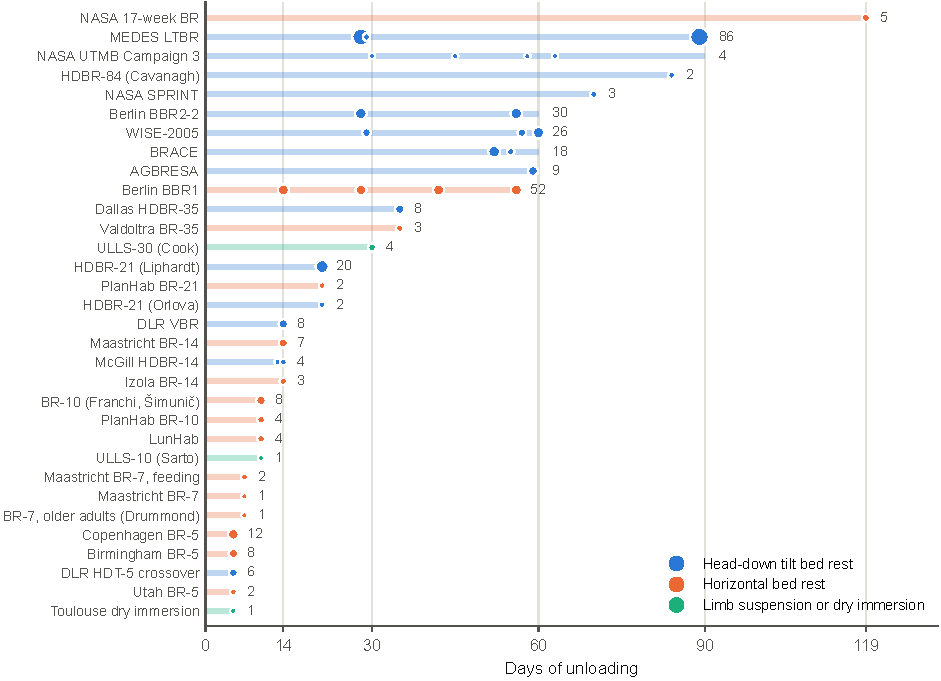
\includegraphics[width=\linewidth]{fig_campaigns}
\caption[The 32 campaigns of the modelling subset]{The 32 campaigns of the modelling subset, ordered by planned
length. Each bar runs to the campaign's planned length of unloading; each dot is a scan day, with area proportional to
the number of rows measured that day; the number is the campaign's rows in subset A. Most campaigns scanned only at
the end; the long campaigns that scanned repeatedly carry most of the within-campaign information about time.}
\label{fig:campaigns}
\end{figure}

\subsection{The modelling subsets}

\Cref{tab:subsets} walks the dataset down to the two modelling subsets. Restricting to rows measured during
unloading removes 264 recovery rows, and the spaceflight and recovery-only campaigns with them; restricting to the
lower limb removes 53 trunk-muscle rows; and the one-tissue-one-row rule removes 79 composite rows whose components
were reported on the same occasion. Of the 346 rows in subset A, 246 are from control arms (30 campaigns) and 100
from countermeasure arms; 42 are whole-segment measurements; 251 are MRI volumes. Subset B removes the whole-segment
rows and with them seven campaigns that report nothing else.

\begin{table}[htbp]
\centering
\caption[From the frozen dataset to the modelling subsets]{From the frozen dataset to the modelling subsets. The
predicates are declared in \file{framework/config.yaml} and applied in this order.}
\label{tab:subsets}
\small
\begin{tabularx}{\linewidth}{@{}Y rrr@{}}
\toprule
Step & Rows & Studies & Campaigns \\
\midrule
\inputtable{generated/tab_subsets.tex}
\bottomrule
\end{tabularx}
\end{table}

\subsection{A first look at the data}

Before any model, the unadjusted control-arm means already show the pattern the models go on to quantify
(\cref{tab:classmeans}): antigravity extensors lose about twice as much as flexors. By family, the plantar flexors
lose most ($-14.7\%$), followed by the evertors ($-12.2\%$), knee extensors ($-8.6\%$), knee flexors ($-7.8\%$),
dorsiflexors ($-7.5\%$), hip adductors ($-4.1\%$) and hip rotators ($-1.3\%$). These means ignore duration, arm,
modality and campaign, and are shown only as a sanity check on the muscle classification.

\begin{table}[htbp]
\centering
\caption[Unadjusted control-arm means by functional class]{Unadjusted mean percentage change of control-arm rows
by functional class (lower-limb rows during unloading, before the one-tissue-one-row rule).}
\label{tab:classmeans}
\small
\begin{tabular}{@{}lrr@{}}
\toprule
Functional class & Rows & Mean change (\%) \\
\midrule
\inputtable{generated/tab_class_means.tex}
\bottomrule
\end{tabular}
\end{table}

\section{Results II: the three tiers}
\label{sec:results-models}

All results in this section are fitted on \code{dataset\_v1.1} with unloading measured at the day of the scan.

\subsection{Tier 1: the duration--response}
\label{sec:results-tier1}

\paragraph{The shape of the curve} The three duration forms fit the 346 rows of subset A almost equally well
(\cref{tab:forms}): the logarithmic, saturating and spline forms lie within 1.3 AIC points of one another, far
inside the 4-point margin the headline rule required for another form to displace the saturating one. The data
therefore establish that loss accumulates along a curved path, but not \emph{which} curve. The spline shows no shape
the parametric forms miss ($\Delta\mathrm{AIC} = -0.2$). By the declared rule the saturating form is the headline.

\begin{table}[htbp]
\centering
\caption[Tier 1: the three duration forms]{Tier 1, subset A (346 rows, 32 campaigns): the three duration forms.
$\Delta$AIC is relative to the headline saturating form; $k$ counts fixed effects, the four variance components
and, for the saturating form, $\tau$. Intervals are 95\% cluster-robust ($t_{31}$).}
\label{tab:forms}
\small
\begin{tabularx}{\linewidth}{@{}L{3.6cm} r r r Y@{}}
\toprule
Form & AIC & $\Delta$AIC & $k$ & Duration term \\
\midrule
\inputtable{generated/tab_tier1_forms.tex}
\bottomrule
\end{tabularx}
\end{table}

\paragraph{How fast and how far} Under the logarithmic form, muscle size falls by 2.99\pp{} for every doubling of
days (95\% CI 2.53 to 3.44). Under the saturating form, the time constant is 60 days---the profile likelihood turns
over inside the declared grid---and the eventual loss is $-17.3\%$ ($-20.9$ to $-13.7$) for the reference scenario.
By day 119, the longest observation, the curve has covered 86\% of the way to that plateau, so the plateau is an
estimate at the edge of the data rather than far beyond it. \Cref{fig:duration} shows the curve with the
control-arm observations, and \cref{tab:curve} its values at selected days.

\begin{figure}[htbp]
\centering
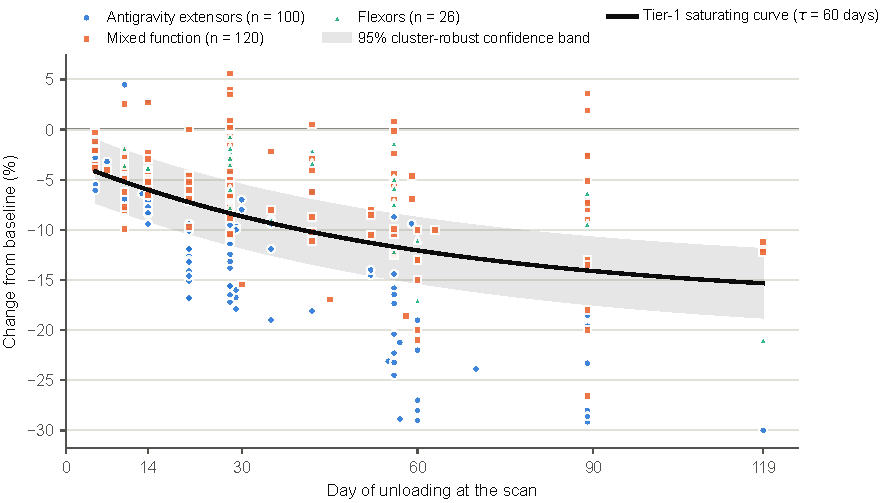
\includegraphics[width=\linewidth]{fig_duration}
\caption[Duration--response: control-arm observations and the tier-1 curve]{Duration--response. Points are the
246 control-arm rows of subset A (30 campaigns), placed at the day of the scan and coloured by functional class. The
line is the tier-1 saturating curve for the reference scenario (a control arm, knee extensors, CT cross-sectional
area, not a composite) with its 95\% cluster-robust band. The scatter around the curve is dominated by which muscle
was measured: antigravity extensors lie mostly below it, flexors and mixed muscles above.}
\label{fig:duration}
\end{figure}

\begin{table}[htbp]
\centering
\caption[Tier 1: the fitted curve at selected days]{The tier-1 saturating curve at selected days for the reference
scenario, with 95\% cluster-robust confidence intervals.}
\label{tab:curve}
\footnotesize
\setlength{\tabcolsep}{4pt}
\begin{tabular}{@{}l cccccc@{}}
\toprule
\inputtable{generated/tab_curve.tex}
\bottomrule
\end{tabular}
\end{table}

\paragraph{Where the variance sits} \Cref{tab:variance} decomposes the variance. In subset A, 54\% is residual,
30\% lies \emph{between muscles within a campaign}, 11\% between campaigns and 4\% between papers reporting the same
campaign. The 30\% is the quantitative case for the second claim of the project: once duration is accounted for,
which muscle is measured matters more than which campaign measured it.

\begin{table}[htbp]
\centering
\caption[Tier 1: variance components]{Tier 1 variance components (squared percentage points) and their share of
the total.}
\label{tab:variance}
\small
\begin{tabular}{@{}lcccc@{}}
\toprule
Model & Campaign & Study within campaign & Muscle within campaign & Residual \\
\midrule
\inputtable{generated/tab_variance.tex}
\bottomrule
\end{tabular}
\end{table}

\paragraph{Other terms} In subset A, countermeasure arms lose 3.43\pp{} less than control arms (95\% CI 1.68 to
5.18, $p < 0.001$). Relative to CT cross-sectional area, DXA lean mass shows 4.75\pp{} less loss (0.05 to 9.45,
$p = 0.048$) and ultrasound thickness 5.95\pp{} less (0.61 to 11.29, $p = 0.030$), while MRI volume differs by only
0.49\pp{} ($p = 0.72$); a curve drawn for MRI volume, the dominant measurement, would therefore sit about half a
percentage point above the reference curve. The composite flag and the whole-segment family carry no detectable
effect. All coefficients are listed in \cref{app:fixed}.

\subsection{Tier 1: muscle-specific vulnerability}
\label{sec:results-ranking}

The ranking model, fitted on the 304 named-muscle rows of subset B (25 campaigns), orders the muscle families by
their fitted change at day 60 for a control arm (\cref{tab:ranking,fig:ranking}). The plantar flexors lose most,
$-15.8\%$ ($-18.9$ to $-12.7$), significantly more than the knee extensors ($-5.69$\pp, $p = 0.001$). The knee
extensors, knee flexors and dorsiflexors form a middle group near $-10\%$; the hip adductors, extensors and rotators
lose significantly less than the knee extensors, the hip rotators least of all ($-1.9\%$).

\begin{table}[htbp]
\centering
\caption[Tier 1: muscle-family ranking at day 60]{Tier 1 muscle-family ranking, subset B (304 rows, 25 campaigns):
fitted change at day 60 for a control arm, and contrast with the reference family (knee extensors). Intervals are
95\% cluster-robust ($t_{24}$). Hip abductors and hip rotators each rest on a single campaign.}
\label{tab:ranking}
\small
\begin{tabular*}{\linewidth}{@{\extracolsep{\fill}}l r r c c r@{}}
\toprule
Family & Rows & Campaigns & \makecell{Change at day 60,\\ \% (95\% CI)} & \makecell{vs.\ knee extensors,\\ pp (95\% CI)} & $p$ \\
\midrule
\inputtable{generated/tab_ranking.tex}
\bottomrule
\end{tabular*}
\end{table}

\begin{figure}[htbp]
\centering
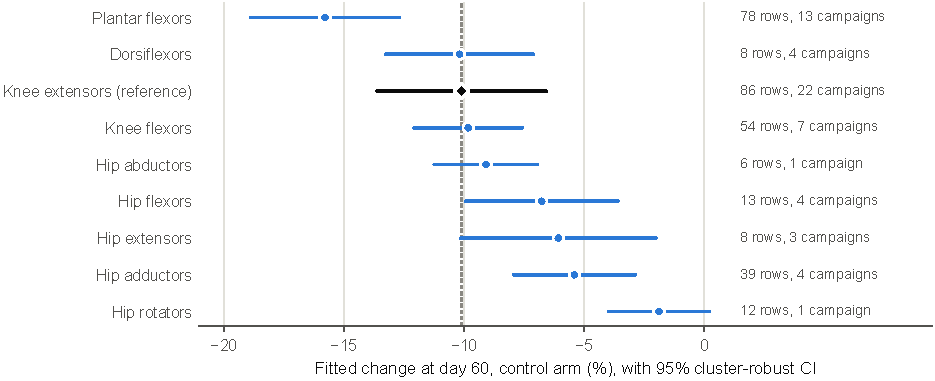
\includegraphics[width=\linewidth]{fig_ranking}
\caption[Muscle-family ranking at day 60]{Muscle-family ranking at day 60 for a control arm, with 95\%
cluster-robust intervals, from the tier-1 ranking model on subset B. The dashed line marks the reference family.
Rows and campaigns are shown for each family because two families rest on a single campaign.}
\label{fig:ranking}
\end{figure}

\paragraph{The antigravity contrast} Because every contrast in \cref{tab:ranking} inherits the uncertainty of the
reference, the comparison that carries the physiological claim is reported on its own: plantar flexors against
dorsiflexors, the antagonist pair at the ankle, is $-5.60$\pp{} (95\% CI $-9.13$ to $-2.07$, $p = 0.003$), computed
from the coefficient difference so that no choice of reference can change it. The ordering survives adjustment for
duration, arm and modality.

\paragraph{Countermeasures} In the ranking model, countermeasure arms lose 3.73\pp{} less than control arms (95\% CI
1.54 to 5.93, $p = 0.002$). This is the first countermeasure effect the project has estimated rather than described;
it pools every countermeasure type and says nothing about which works best.

\subsection{Sensitivity analysis S6: does the weighting matter?}
\label{sec:results-s6}

The primary analysis weights rows by the number of participants analysed. The classical alternative, inverse-variance
weighting, needs a dispersion \emph{of the change}, which only 161 of the 346 rows in subset A, from 8 of the 32
campaigns, carry; most papers print the spread of the baseline or nothing. \Cref{tab:s6} compares the two schemes on
the same rows. The restriction to rows with a change dispersion moves the duration coefficient by 0.3\pp{} and the
weighting scheme by another 0.9\pp, with overlapping intervals throughout: on this literature the scheme barely
matters. The finding that belongs in the methods is the other one: inverse-variance weighting is unavailable as a
primary scheme, because only eight campaigns carry what it needs.

\begin{table}[htbp]
\centering
\caption[Sensitivity analysis S6]{Sensitivity analysis S6. The duration coefficient is the saturating term of the
tier-1 model; the error is out-of-campaign and campaign-weighted. From \file{results/sensitivity.md}.}
\label{tab:s6}
\small
\begin{tabularx}{\linewidth}{@{}Y l r r c r@{}}
\toprule
Analysis & Weights & Rows & Campaigns & Duration coefficient (95\% CI) & MAE (pp) \\
\midrule
Primary: every row & participants & 346 & 32 & $-14.25$ ($-16.40$ to $-12.11$) & 3.34 \\
Rows with a dispersion of the change & participants & 161 & 8 & $-14.51$ ($-15.61$ to $-13.42$) & 2.67 \\
S6: the same rows & inverse variance & 161 & 8 & $-13.60$ ($-16.69$ to $-10.50$) & 2.82 \\
\bottomrule
\end{tabularx}
\end{table}

\subsection{The duration-only baseline}
\label{sec:results-baseline}

Fitted inside the leave-one-campaign-out loop, the logarithmic curve is the best of the three baseline forms, with
an out-of-campaign MAE of 3.16\pp{} (95\% CI 2.44 to 3.93); the saturating form follows closely (3.19\pp) and the
straight line is worst (3.40\pp), which is the evidence that the relationship is curved rather than assumed to be
(\cref{tab:models}). All three forms already meet the 4\pp{} target before any model family is fitted. Their pooled
$R^2$ is low (0.07 to 0.14): duration alone predicts the average loss at a given day, but explains little of the
row-to-row variation, because that variation is mostly which muscle was measured. Averaged over all muscles in
subset A, the fitted saturating baseline has a time constant of 35 days and an eventual loss of $-13.0\%$; the
whole-segment and composite rows pull that average towards the less affected tissue, which is why the tier-1 model
with muscle terms, not the baseline, answers the question for a particular muscle.

\subsection{Tier 2: the comparative machine-learning families}
\label{sec:results-tier2}

\begin{keybox}{Tier 2 is a null result}
No family beats the duration-only curve (\cref{tab:models,fig:models}). The best, a random forest, scores 3.18\pp{}
against the curve's 3.16\pp{}; the others are between 3.7\% and 5.9\% worse. The plan set the bar at a 15\% relative
improvement and pre-committed to reporting the outcome either way. This is rung~B of the project's fallback ladder.
A pretrained tabular neural network, TabPFN, added afterwards as a fifth family, does not beat the curve either
(3.22\pp, 2.1\% worse).
\end{keybox}

\begin{table}[htbp]
\centering
\caption[Tier 2: out-of-campaign error of the baseline and the four families]{Out-of-campaign error of the
duration-only baseline in its three forms and of the four tier-2 families, subset A, 32 leave-one-campaign-out
folds. MAE and RMSE are campaign-weighted; the interval is a campaign bootstrap; ``vs.\ baseline'' is the relative
MAE change against the logarithmic curve (negative = worse); $R^2$ is pooled over out-of-fold predictions. The last
column names the campaign with the largest error and that error. TabPFN was added after the four families' result
was known and was run in its own environment (\cref{sec:tier2}).}
\label{tab:models}
\footnotesize
\begin{tabular*}{\linewidth}{@{\extracolsep{\fill}}l c c c c c l@{}}
\toprule
Model & \makecell{MAE\\ (pp)} & 95\% CI & RMSE & \makecell{vs.\\ baseline} & $R^2$ & Worst campaign (MAE) \\
\midrule
\inputtable{generated/tab_models.tex}
\bottomrule
\end{tabular*}
\end{table}

\begin{figure}[htbp]
\centering
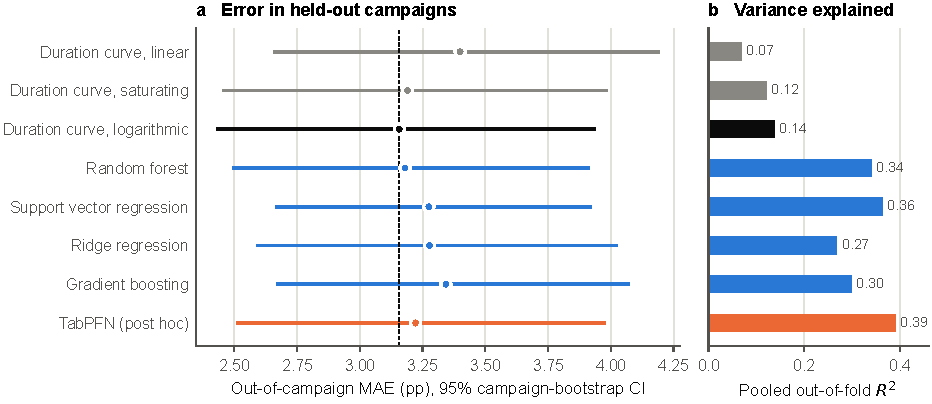
\includegraphics[width=\linewidth]{fig_models}
\caption[Tier 2 against the duration curve]{Tier 2 against the duration curve. (a)~Out-of-campaign MAE with 95\%
campaign-bootstrap intervals; the dashed line is the logarithmic curve. (b)~Pooled out-of-fold $R^2$. Blue: the
four declared families; orange: TabPFN, added post hoc. The flexible families explain two to three times more
variance than the curve, yet do not convert it into lower error.}
\label{fig:models}
\end{figure}

The informative part is panel~b of \cref{fig:models}. Pooled $R^2$ rises from 0.14 for the curve to 0.27--0.36
once muscle identity enters: the flexible families do find real structure, but they do not convert it into a lower
absolute error, because the residual is dominated by between-campaign differences that no column in the dataset
explains. The worst folds show where: a 21-day campaign with site-resolved thigh measurements (HDBR-21, Liphardt;
7.8--7.9\pp) for three families, and WISE-2005, 60 days of bed rest in women only, for ridge regression (8.6\pp).

\paragraph{The pretrained network} TabPFN, the post-hoc fifth family, scores 3.22\pp{} (95\% CI 2.51 to 3.97), 2.1\%
worse than the curve and second of the five families behind the random forest. Its pooled $R^2$ of 0.39 is the highest
of any tier-2 model: a network pretrained on millions of synthetic tables, conditioning on the training campaigns in
context, finds the muscle structure as the tuned families do, and like them does not turn it into lower error in a
campaign it has not seen. Its worst campaigns are the same ones: HDBR-21 (Liphardt; 7.56\pp) and WISE-2005 (7.34\pp).
An earlier run of the same family, on \code{dataset\_v1.0} and the campaigns' planned lengths, had scored 3.25\pp{} with
a pooled $R^2$ of 0.03, behaving like a duration-only curve; on the day of the scan it behaves like the other families.
Either way the conclusion is the same, and it now rests on five families of very different kinds, from penalised
regression to a pretrained transformer.

\paragraph{Importance} SHAP values on the random forest identify two stable features (\cref{tab:importance}): the
duration term reaches the top three in 29 of 32 folds (91\%) and the plantar-flexor indicator in 28 (88\%). The third
place alternates between the countermeasure arm (59\%) and the composite flag (53\%), so the declared criterion---the
same top three in 80\% of folds---is missed. The flexible models lean on exactly the two variables the tier-1 model
estimates with intervals, which is the consistency the importance analysis was meant to check; it is not evidence of
cause.

\begin{table}[htbp]
\centering
\caption[Tier 2: stability of feature importance]{Stability of SHAP importance for the random forest across the 32
folds: how often each feature reaches the top three, and its mean absolute SHAP value. Features never in the top three
are omitted.}
\label{tab:importance}
\small
\begin{tabular}{@{}lccc@{}}
\toprule
Feature & Folds in top three & Share & Mean $|$SHAP$|$ \\
\midrule
\inputtable{generated/tab_importance.tex}
\bottomrule
\end{tabular}
\end{table}

\subsection{Tier 3: the probabilistic forecast}
\label{sec:results-tier3}

The first run sent 430 requests, the largest of 26,390 input tokens. \Cref{tab:forecast} reports both arms against
their references on identical metrics.

\begin{table}[htbp]
\centering
\caption[Tier 3: forecast accuracy and calibration]{Tier 3 against its references. MAE and CRPS in percentage
points, campaign-weighted, with a campaign-bootstrap interval for the MAE; the log score is per row (lower is better);
coverage and mean width (pp) of the most probable 50\% and 80\% ranges. $^\dagger$ the arm's reference.}
\label{tab:forecast}
\small
\begin{tabularx}{\linewidth}{@{}Y c c c c c c c@{}}
\toprule
Model & MAE & 95\% CI & CRPS & Log score & 50\% range & 80\% range & $R^2$ \\
\midrule
\inputtable{generated/tab_forecast.tex}
\bottomrule
\end{tabularx}
\end{table}

\paragraph{Without history} \Jev's error is 2.71\pp{} against the curve's 3.13\pp.\footnote{The curve scores
3.13\pp{} here and 3.16\pp{} in \cref{tab:models} because here its point is the mean of its forecast distribution, the
same definition used for the model's point.} Paired by campaign, the model's error is lower by 0.42\pp{} (95\% CI
0.13 to 0.73), and it is closer in 20 of the 32 campaigns (\cref{fig:jevcampaigns}). This is the first advantage over
the duration curve in the project whose paired interval excludes zero, and the pooled $R^2$ of 0.43 is about three
times the curve's (\cref{fig:jevscatter}). Against the declared bars, however, the MAE improvement is 13.3\%, short
of the 15\% required; the CRPS improvement, 17.7\%, meets its bar; and the 80\% ranges contain the truth only 62\% of
the time, so they may not be called 80\% ranges. The log score says the same from the other side: it is worse than
the curve's (2.84 against 2.29) despite the better CRPS, because when the model is wrong it has placed almost no
probability where the truth landed.

\paragraph{With history} Forecasting the change since the previous scan on 84 rows from five campaigns, \Jev{}
reaches 2.84\pp{} against 3.21\pp{} for the last scan plus the curve's step, a paired gain of 0.37\pp{} (0.03 to
0.75) in four of the five campaigns. The MAE improvement (11.5\%) misses its bar, the CRPS is 2.2\% worse than the
reference, and the ranges are badly overconfident: 2.8\pp{} wide, they contain the truth 38\% of the time. With five
campaigns, every interval on this arm rests on a bootstrap over five values and is indicative only.

\begin{figure}[htbp]
\centering
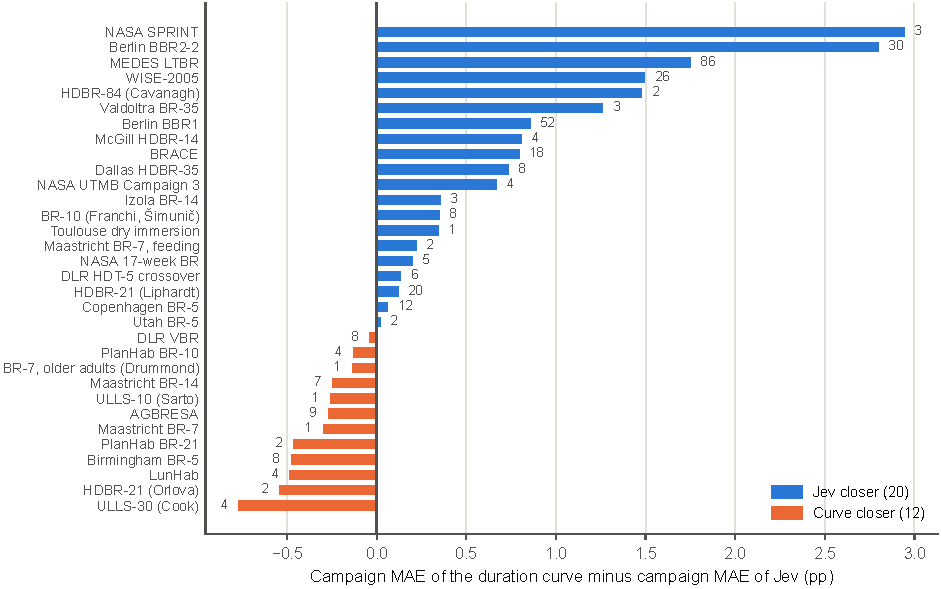
\includegraphics[width=\linewidth]{fig_jev_campaigns}
\caption[Tier 3: gain by held-out campaign]{Tier 3 without history: the duration curve's campaign MAE minus \Jev's,
for each held-out campaign (positive = \Jev{} closer). The number beside each bar is the campaign's rows. More than
half of the total gain comes from three long, multi-muscle MRI campaigns---NASA SPRINT, Berlin BBR2-2 and MEDES
LTBR---which are also among the most published campaigns in the field.}
\label{fig:jevcampaigns}
\end{figure}

\begin{figure}[htbp]
\centering
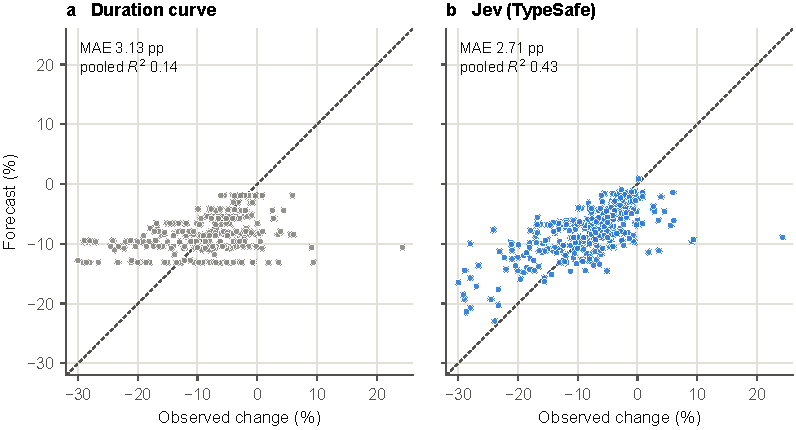
\includegraphics[width=\linewidth]{fig_jev_scatter}
\caption[Tier 3: forecast against observed value]{Forecast against observed change for all 346 rows of subset A,
each forecast made with its campaign held out. (a)~The duration curve predicts nearly one value per scan day. (b)~\Jev{}
follows the between-muscle spread, which is where its gain comes from; both regress towards the mean at the extremes.
Dashed line: identity.}
\label{fig:jevscatter}
\end{figure}

\subsection{Tier 3: is the gain signal or recognition?}
\label{sec:results-ablation}

Because more than half of the gain came from three much-published campaigns, the ablations and the recognition probe
were declared and run (1,280 new answers). \Cref{tab:ablation} and panel~a of \cref{fig:jevchecks} report them.

\begin{table}[htbp]
\centering
\caption[Tier 3: ablations]{Tier 3 ablations on the arm without history (346 rows, 32 campaigns). The paired gain is
over the duration curve; the change is relative to the full run (negative = worse). Intervals are campaign bootstraps.}
\label{tab:ablation}
\footnotesize
\begin{tabular*}{\linewidth}{@{\extracolsep{\fill}}l c c c c c c@{}}
\toprule
Variant & MAE & CRPS & \makecell{80\%\\ cover} & \makecell{Paired gain,\\ pp (95\% CI)} & \makecell{Change vs.\ full,\\ pp (95\% CI)} & Closer \\
\midrule
\inputtable{generated/tab_ablation.tex}
\bottomrule
\end{tabular*}
\end{table}

\paragraph{Against the reading rules}
\begin{itemize}
  \item \textbf{The generic variant keeps the gain}: 0.30\pp{} (0.01 to 0.62), at least half of the full run's 0.42\pp{}
        with an interval above zero; its difference from the full run, $-0.11$\pp, has an interval that includes zero.
        The gain does not need anything that identifies a study.
  \item \textbf{The model reads the reference data}: with the other campaigns' values shuffled, the gain becomes a loss
        of 1.25\pp; without any reference data the model is far worse than the curve (5.85 against 3.13\pp).
  \item \textbf{Recognition is not a live explanation} (\cref{fig:recognition}). The model places a mean probability
        of 0.14 on the true campaign, against 0.08 by chance, and names it first on 19\% of rows. Three campaigns pass
        the recognition bar---NASA SPRINT and AGBRESA (named first on 67\% of their rows) and VBR (50\%)---but of the
        three that carry most of the gain only SPRINT is recognised; for BBR2-2 and MEDES LTBR the model's commonest
        answer is ``none of these''. Recognition and gain correlate at $\rho = 0.37$ ($p = 0.26$, 11 campaigns).
\end{itemize}
By the declared table this is the first case: \emph{tier 3's point forecasts may be quoted as a result}, with the
caveats of \cref{sec:results-tier3}. The campaign-level errors point the same way. A model recalling published numbers
should do best without reference data on the campaigns it can name; it does not, being worse than the curve on
AGBRESA (6.13 against 2.95\pp) and VBR (5.73 against 0.95\pp). SPRINT is the exception (4.80 against 5.92\pp) and the
one place recognition may contribute, but the generic variant, which gives the model nothing to recognise SPRINT by,
still beats the curve there (3.79 against 5.92\pp). The one campaign no paper reports, UTMB Campaign~3, computed from
NASA's raw archive, also favours the model (0.67\pp{} gain, four rows).

\begin{figure}[htbp]
\centering
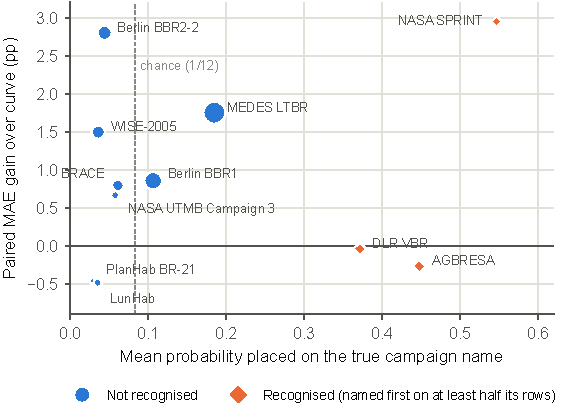
\includegraphics[width=0.7\linewidth]{fig_recognition}
\caption[Tier 3: recognition probe]{Recognition probe, 11 campaigns with proper names. Horizontal: mean probability
the model places on the true campaign name when shown the description the forecast uses; vertical: the campaign's
paired gain over the curve. Marker area is proportional to rows. Two of the three campaigns carrying most of the gain
(BBR2-2, MEDES LTBR) are not recognised.}
\label{fig:recognition}
\end{figure}

\subsection{Tier 3: does it hold up?}
\label{sec:results-validation}

The validation battery added 1,195 answers and 20 repeats past the cache (\cref{tab:validation}, \cref{fig:jevchecks}).

\begin{table}[htbp]
\centering
\caption[Tier 3: validation battery]{Tier 3 validation battery, leave-one-campaign-out throughout. MAE in pp for
\Jev{} and for the arm's reference; paired gain over the reference and change from the full run with 95\%
campaign-bootstrap intervals. On the history arm each interval rests on five campaigns.}
\label{tab:validation}
\footnotesize
\begin{tabular*}{\linewidth}{@{\extracolsep{\fill}}l c c c c@{}}
\toprule
Run & \makecell{\Jev{}\\ MAE} & \makecell{Reference\\ MAE} & \makecell{Paired gain,\\ pp (95\% CI)} & \makecell{Change vs.\ full,\\ pp (95\% CI)} \\
\midrule
\inputtable{generated/tab_validation.tex}
\bottomrule
\end{tabular*}
\end{table}

\begin{figure}[htbp]
\centering
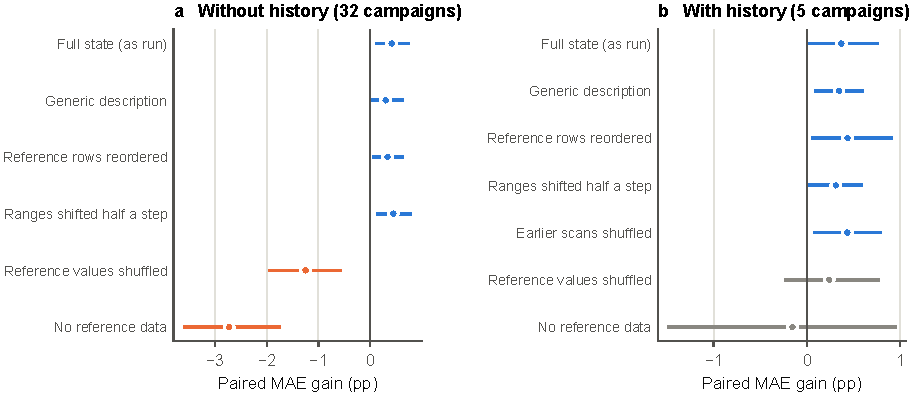
\includegraphics[width=\linewidth]{fig_jev_checks}
\caption[Tier 3: the gain under every check]{Paired MAE gain of \Jev{} over each arm's reference under every
ablation and presentation check, with 95\% campaign-bootstrap intervals. Blue: interval above zero; orange: below
zero; grey: spans zero. (a)~Without history the gain survives every change of presentation and the removal of
identifying detail, and collapses when the reference data are shuffled or removed. (b)~With history the gain is
unchanged when the campaign's own earlier scans are shuffled.}
\label{fig:jevchecks}
\end{figure}

\paragraph{Against the reading rules}
\begin{itemize}
  \item \textbf{Robust to presentation: yes, on both arms.} Without history the MAE moves by 3\% under reordering and
        1\% under shifted ranges, and the gain keeps an interval above zero under both (0.34 and 0.45\pp). On the
        history arm both moves are 2\% and the gain keeps its sign.
  \item \textbf{Consistent: no, by the letter of the rule.} None of the 20 repeated requests returned identical
        probabilities. The probabilities moved by 0.034 on average (0.09 at most), the forecasts by 0.17\pp{} on
        average (0.48 at most), the most likely range held in 18 of 20, and the error on the repeated rows went from
        2.456 to 2.479\pp. Run-to-run variation is of the order of the differences between presentation runs and far
        below the 0.42\pp{} gain.
  \item \textbf{Reads the earlier scans: no.} Shuffling the held-out campaign's earlier values leaves the error where
        it was ($+0.06$\pp, interval across zero).
  \item \textbf{Reads the other campaigns on the history arm: not shown.} Both reference ablations are worse in their
        point estimates, by 0.13 and 0.52\pp, but on five campaigns neither interval clears zero.
  \item \textbf{The earlier scans help---strongly, but not through the model.} On the same 84 rows the model's error
        falls from 5.83 to 2.84\pp{} when it forecasts the change since the last scan rather than the level (paired
        2.98\pp, 1.54 to 5.51), and the baselines' from 7.27 to 3.21\pp{} (4.06\pp, 2.52 to 5.99). What the earlier
        scans supply is the anchor, and the code supplies it by adding the forecast change to the last scan.
\end{itemize}
Of the three conditions for calling tier 3 working rather than lucky, the one that carries the quoted number holds:
the result without history survives both presentation checks and its run-to-run variation is far smaller than the
gain. The other two fail and are reported as failing. The tier-3 number is therefore quoted from the arm without
history, with the note that repeated runs differ slightly; nothing is claimed about the model using a campaign's
earlier scans.

\subsection{The effect of correcting the time axis}
\label{sec:results-correction}

\Cref{tab:correction} records what changed when tiers 1 and 2 moved from the campaign's planned length to the day of
the scan (\cref{sec:target}). The fit improved by about 65 AIC points on identical rows, the plainest evidence that
the scan day is the right exposure; the time constant moved from the edge of the declared grid to its interior; and
the share of variance between muscles rose. What matters for the conclusions did not change: the duration forms remain
indistinguishable, the ranking keeps its order, and no tier-2 family beats the curve. Tier 3 was fitted on the scan
day from the start.

\begin{table}[htbp]
\centering
\caption[The time-axis correction]{Results fitted on the campaign's planned length (first runs, superseded) and on the
day of the scan (reported). Values for the planned length are as recorded in \file{framework/DESIGN.md}, section 9.4.}
\label{tab:correction}
\small
\begin{tabularx}{\linewidth}{@{}Y c c@{}}
\toprule
Result & Planned length & Day of the scan \\
\midrule
Tier 1, saturating form, AIC on the same 346 rows & 2152.3 & \textbf{2085.9} \\
Residual variance & 17.7 & \textbf{13.8} \\
Loss per doubling of days, logarithmic form (pp) & $-2.41$ ($-3.26$ to $-1.56$) & \textbf{$-$2.99} ($-3.44$ to $-2.53$) \\
Saturating time constant & 90 days, at the edge of the grid & \textbf{60 days}, inside it \\
Eventual loss, saturating form (\%) & $-19.9$ ($-24.8$ to $-15.0$) & \textbf{$-$17.3} ($-20.9$ to $-13.7$) \\
Share of variance between muscles within a campaign & 23\% & \textbf{30\%} \\
Baseline (logarithmic), out-of-campaign MAE & 3.21\pp & \textbf{3.16\pp} \\
Baseline pooled $R^2$ & 0.03 & \textbf{0.14} \\
Best tier-2 family against the baseline & SVR, $-0.4\%$ & \textbf{Random forest, $-$0.7\%} \\
Tier-2 pooled $R^2$ & 0.10--0.22 & \textbf{0.27--0.36} \\
Features stable in the top three ($\geq$80\% of folds) & duration only, at 69\% & \textbf{duration (91\%), plantar flexors (88\%)} \\
\bottomrule
\end{tabularx}
\end{table}

\subsection{Assessment against the declared criteria}
\label{sec:results-criteria}

\Cref{tab:assessment} sets every criterion declared before modelling, and every bar declared for tier 3, against
its outcome. Of the six criteria for tiers 1 and 2, the three that were allowed to fail split one met and two missed;
of the three blocking criteria, two are met and the physiological sign-off is outstanding.

\begin{table}[H]
\centering
\caption[Assessment against the declared criteria]{Assessment against the criteria of \cref{tab:criteria} and the
tier-3 bars.}
\label{tab:assessment}
\small
\begin{tabularx}{\linewidth}{@{}L{4.8cm} L{2.2cm} Y@{}}
\toprule
Criterion & Outcome & Evidence \\
\midrule
Out-of-campaign MAE $\leq$ 4\pp & Met & Every baseline form and every family, 3.16--3.40\pp \\
Best model $\geq$ 15\% better than baseline & Not met & Best family $-0.7\%$; null result reported \\
\quad TabPFN, post hoc, against the same bar & Not met & $-2.1\%$; pooled $R^2$ 0.39 \\
SHAP top-3 stability $\geq$ 80\% & Not met & Top two stable (91\%, 88\%); third place 59\% \\
Leakage audit & Met & Disjointness asserted in every fold; the assertion is tested against a bad split \\
Reproducibility & Met & One command rebuilds every result; 234 tests pass; tier 3 rebuilt from its cache \\
Physiological sign-off & \textbf{Outstanding} & Muscle classification and fitted relationships await the scientific lead \\
\addlinespace
Tier 3, MAE $\geq$ 15\% better & Not met & 13.3\% without history, 11.5\% with \\
Tier 3, CRPS $\geq$ 15\% better & Met without history & 17.7\%; with history 2.2\% worse \\
Tier 3, 80\% coverage in 70--90\% & Not met & 62\% and 38\%: ranges overconfident \\
Tier 3, leakage and reproducibility & Met & Assertions on every request; cache rebuild without API calls \\
\bottomrule
\end{tabularx}
\end{table}

\section{Discussion}
\label{sec:discussion}

\subsection{Principal findings}

Four statements are supported by the evidence, listed in order of how well it supports them.

\begin{enumerate}
  \item \textbf{Muscle loss during bed rest follows a curved, not linear, path}: about 3\pp{} per doubling of days
        (95\% CI 2.5 to 3.4), with the reference curve at $-12\%$ by day 60 and $-15\%$ by day 119. The corpus
        cannot say \emph{which} curve: logarithmic, saturating and spline forms are indistinguishable.
  \item \textbf{Which muscle is measured matters more than anything else in the dataset.} Thirty per cent of the
        variance lies between muscles within a campaign; plantar flexors lose 5.7\pp{} more than knee extensors
        and 5.6\pp{} more than their antagonists, the dorsiflexors; antigravity extensors lose roughly twice what
        flexors lose. The flexible models of tier~2 lean on the same two variables.
  \item \textbf{At 32 campaigns, tabular machine learning adds nothing to a simple curve.} The four families find
        the muscle structure---pooled $R^2$ doubles or triples---but do not convert it into lower out-of-campaign
        error. That is a statement about how much signal the published literature contains, not about the
        algorithms.
  \item \textbf{A model that reads the other campaigns' data in context adds a little.} The language-model forecast
        is 0.42\pp{} more accurate than the curve, survives the removal of study-identifying detail and every
        presentation check, and is not explained by recognition of published campaigns. It was not pre-registered,
        it misses its declared bar and its ranges are overconfident; it is a finding to report, not the headline.
\end{enumerate}

\subsection{The duration--response}

The clearest single result is negative about shape and positive about magnitude. A straight line in days is the worst
of the three baseline forms, and the curvature is real: roughly 40\% of the loss the reference curve reaches by day
119 has already occurred by day 14 ($-6.0\%$ of $-15.3\%$). What the data cannot do is choose between a curve that
keeps falling with the logarithm of time and one that approaches a plateau. The 32 campaigns are concentrated at 5--21
and 56--90 days, with a single campaign at 119 days, and both forms pass through that support equally well. The
saturating form was kept as the headline by a rule declared in advance, because its parameters are interpretable---a
time constant of 60 days and an eventual loss of about 17\%---not because the data prefer it. For planning purposes
the honest summary is the curve and its band over the observed range, not the asymptote.

Two properties of the curve should be kept in view when quoting it. It is drawn for one scenario: a control arm, knee
extensors, measured as CT cross-sectional area. For MRI volume it sits about half a percentage point higher, and for
plantar flexors about 5.7\pp{} lower. And it is fitted to group means: it describes what a group of similar people
would lose on average, not what an individual will lose.

\subsection{Muscle-specific vulnerability: mechanical role}

The ranking reproduces, as adjusted coefficients with intervals, the selective vulnerability reported by
muscle-resolved bed-rest studies~\citep{belavy2009,miokovic2012,marusic2021}: the plantar flexors are the most
affected family and the hip rotators and adductors the least. The corpus also offers a partial test of the two usual
explanations. Tibialis anterior, the principal dorsiflexor, is slow-fibre dominant like the soleus~\citep{johnson1973}
but does not carry body weight; if fibre type governed atrophy, the dorsiflexors should lose like the plantar flexors.
They do not: they lose like the knee extensors ($-10.2\%$ against $-10.1\%$ at day 60) and 5.6\pp{} less than the
plantar flexors. The comparison rests on eight dorsiflexor rows from four campaigns and on a classification that has
not yet been signed off, so it is suggestive rather than decisive, but it points towards mechanical role.

The countermeasure effect, 3.7\pp{} less loss in countermeasure arms, pools every countermeasure type, from flywheel
exercise to nutrition. It shows that the dataset can detect a countermeasure effect at all; it cannot say which
countermeasure works, which would need more campaigns per modality than the literature provides.

\subsection{Why flexible learners did not help}

The tier-2 null result is the most important methodological finding of the project, and the explanation is the
sample size. There are 346 rows, but 32 independent campaigns, and the error that matters is the error on a campaign
the model has never seen. Most of what distinguishes one campaign from another---its imaging protocol, its
population, the exact definition of its muscles, its countermeasure dose---is either not recorded in a way that can be
modelled or is perfectly confounded with the campaign itself. The flexible families learn the muscle structure, which
raises pooled $R^2$, but the part of the residual that decides out-of-campaign error is between-campaign, and no
column explains it. With roughly a tenth of the sample size at which flexible learners begin to behave
well~\citep{vanderploeg2014}, this is the expected outcome, and it was prepared for in advance.

The answer this gives to the question ``why not simply use machine learning?'' is a better one than any accuracy
figure would have been: because at this sample size the unit of evidence is the campaign, and the literature holds 32
of them. It also explains why the meta-regression, and not a predictive model, is the right primary tool: it
estimates exactly the structure the learners found, with intervals, and it does not need to predict unseen campaigns
to be useful.

\subsection{What tier 3 does and does not show}

The language-model forecast is the only method in the project whose advantage over the curve has a paired interval
that excludes zero. The ablations establish what the gain does not need---anything that identifies a study---and that
it depends on the reference values: shuffle them and the gain becomes a loss. The recognition probe finds that the
model can name some campaigns, but not the ones carrying the gain. The likeliest reading is that the model does a kind
of case-based reasoning that tier 2 could not: it picks out the reference rows that match the target---same muscle,
same kind of group, a nearby day---and weighs them, where tier 2 received the same information as one-hot columns and
a duration basis. That is an interpretation, not a tested mechanism.

The limits are as clear as the gain. The method was added after the null result; it misses the 15\% bar declared for
it; its ranges are overconfident, so its uncertainty cannot be quoted; its answers vary slightly between identical
requests; and on the history arm it does not use the campaign's earlier scans at all---the benefit of history comes
entirely from the anchor the code supplies. Pretraining exposure to some of these papers cannot be excluded by any
cross-validation.

\subsection{Implications for mission planning}

The results support three statements a countermeasure planner can use, at group level and within the observed range
of 5 to 119 days: that most of the loss seen by four months has accumulated within the first weeks; that the calf's
antigravity muscles are the ones to protect first; and that countermeasure arms in the literature lose measurably
less than controls. They do not support a prediction for an individual astronaut, a statement about actual
microgravity, or a number for day 180. Extrapolation to a six-month transit was specified but has not been run; when
it is, it will be computed from the tier-1 curve only, reported as a prediction interval drawn on the same axes as the
data, and accompanied by the statement that the longest observation is 119 days and that the remainder is an
assumption about curve shape.

\subsection{Reconciliation with the accepted abstract}
\label{sec:abstract-reconciliation}

The accepted abstract was written before the literature search and is the contract for the presentation. The results
confirm its central claims and correct several of its numbers (\cref{tab:abstract}). None of the corrections weakens
the claims; most strengthen the evidence behind them.

\begin{table}[htbp]
\centering
\caption[Reconciliation with the accepted abstract]{The accepted abstract against the results.}
\label{tab:abstract}
\small
\begin{tabularx}{\linewidth}{@{}L{4.6cm} Y@{}}
\toprule
Abstract & Result \\
\midrule
``15 bed-rest and HDBR studies (1992--2025)'' & 52 studies (1992--2026) from 36 independent campaigns; the modelling
  subset holds 41 studies from 32 campaigns \\
``unloading durations of 14--119 days'' & Planned durations and scan days both span 5--119 days \\
Variables include participant characteristics & Recorded, but not modelled: age and sex are almost perfectly confounded
  with the campaign and are reserved for sensitivity analyses S8 and S9 \\
Linear regression, random forest, SVR, gradient boosting & As stated; linear regression is penalised (ridge) \\
Leave-one-study-out cross-validation & Leave-one-\emph{campaign}-out: stricter, because papers from one campaign share
  participants \\
SHAP-based interpretation & Done for the best family; the top two features are stable, the third is not \\
``consistent relationship between duration and loss'' & Confirmed: curved, about $-3$\pp{} per doubling of days \\
Soleus, gastrocnemius and triceps surae most susceptible, ``losses approaching 20--30\% during prolonged bed rest'' &
  Plantar flexors are the most affected family, $-15.8\%$ at day 60 by the model; individual group means reach $-30\%$
  at the longest durations, but the modelled averages do not \\
``Exercise countermeasures consistently associated with reduced muscle loss'' & Countermeasure arms lose 3.7\pp{} less
  (95\% CI 1.5 to 5.9), all countermeasure types pooled \\
Duration and muscle-specific vulnerability as major determinants & Confirmed by tier 1 (variance components,
  coefficients) and by tier-2 importance \\
\bottomrule
\end{tabularx}
\end{table}

\section{Limitations}
\label{sec:limitations}

The limitations are stated in full; several are properties of the literature rather than of the analysis.

\begin{enumerate}
  \item \textbf{Small effective sample.} The modelling subset holds 32 independent campaigns. Every interval is wide
        accordingly, and the covariate budget is about three study-level terms.
  \item \textbf{Clustering and dominance.} One campaign (MEDES LTBR) supplies 40\% of the full dataset and a quarter of
        the modelling subset; 15 campaigns contribute five rows or fewer. Campaign weighting and campaign-level
        validation mitigate this, but the must-show sensitivity analysis that drops the largest campaign (S2) has not
        been run.
  \item \textbf{Search coverage.} The search starts in 2013; older work enters only through a convenience corpus of
        nine papers. Embase was not searched, 1,023 records were not screened in the time available, and 19 included
        studies report their results only as charts without a baseline.
  \item \textbf{No human double extraction.} The extraction was verified against the sources with AI assistance, and
        the pre-search corpus rows were not verified by a second person at all.
  \item \textbf{Heterogeneous measurements in one target.} MRI volume, CT and MRI cross-sectional area, DXA lean mass
        and ultrasound thickness are treated as one target with a modality term; the MRI-only sensitivity analysis
        (S4) is outstanding. The measurement site along a muscle, which matters~\citep{miokovic2012}, is ignored in
        the primary model, and 547 rows do not state which leg was imaged.
  \item \textbf{Mixed granularity and two estimators.} Composites and components coexist, resolved by a rule whose
        opposite (S1) has not been run; the target mixes the printed mean of individual changes with a value
        recomputed from group means.
  \item \textbf{Publication bias} is plausible in this literature and cannot be quantified with 32 campaigns.
  \item \textbf{Bed rest is an analogue.} Nothing here establishes that the coefficients transfer to microgravity;
        the 14 spaceflight rows are too few to test it and eight of them are lumbar multifidus.
  \item \textbf{No data beyond 119 days}, and a single campaign at 119 days.
  \item \textbf{Mostly young men.} 347 of the 425 lower-limb unloading rows come from men-only groups and 38 from
        older adults, in six campaigns.
  \item \textbf{Group means, not individuals.} Every row is an arm mean; nothing can be said about individual
        susceptibility.
  \item \textbf{The NASA campaign is thin.} Three of its four in-bed-rest occasions rest on one participant.
  \item \textbf{Unsigned classification.} The muscle classification awaits physiological sign-off, a blocking
        condition for quoting coefficients by class.
  \item \textbf{Assumptions of the model.} Campaigns are assumed independent of one another; missing dispersions and
        ages are assumed uninformative; the tier-2 families were fitted unweighted.
  \item \textbf{Tier 3} is post hoc, overconfident, not bit-reproducible, and exposed to possible pretraining on the
        source papers.
  \item \textbf{Most sensitivity analyses are outstanding}, including the three declared as must-show.
\end{enumerate}

\section{Status of the work and remaining tasks}
\label{sec:outstanding}

The internal schedule placed the modelling hard stop on 21 September 2026; the report and slides follow, with the
upload deadline on 10 October and the presentation on 15 or 16 October. The following items remain, in order of
priority.

\begin{enumerate}
  \item \textbf{Sensitivity analyses S1, S2 and S4} (composite-first resolution, without MEDES LTBR, MRI volume only),
        declared as must-show in this report; then the remaining analyses where they would change a conclusion.
  \item \textbf{Physiological sign-off} of \file{data/muscle\_map.csv} and of the fitted relationships by the
        scientific lead---a blocking criterion, and a line edit in one file.
  \item \textbf{The 180-day extrapolation} with a prediction interval, as a clearly caveated backup result.
  \item \textbf{Recalibration of tier 3's ranges} by a rule declared in advance, if its uncertainty is to be quoted.
  \item \textbf{Reconcile the PRISMA counts} at the full-text stage with the final extraction.
  \item \textbf{Close P3 and P4 formally}: tag the results and merge the branch stack ending at \ReportBranch{} into
        \code{main}.
  \item \textbf{Repository housekeeping before publication}: add a licence (code and dataset need different ones),
        remove the full-text digests that reproduce copyrighted text, acknowledge NASA as a data source, check the
        terms under which tier 3's cached answers may be published, and obtain both leads' agreement to the one
        schema change in v1.1.
  \item \textbf{Two data checks}: two countermeasure-arm rows carry \code{cm\_modality = none}, and the figure-derived
        extraction table fails the validator unless run in partial mode (23 rows lack sex or age).
  \item \textbf{Author instructions} from the organisers (slide format, time limit, disclosure requirements), still
        outstanding.
\end{enumerate}

\section{Conclusions}
\label{sec:conclusions}

The published bed-rest literature, organised into one frozen dataset of 742 comparisons from 52 studies and 36
campaigns, supports a quantified duration--response---about 3 percentage points of muscle per doubling of days of
unloading, curved rather than linear---and a muscle-specific vulnerability led by the plantar flexors, with
countermeasure arms losing measurably less. Tested honestly, by holding out whole campaigns, four machine-learning
families add nothing to a simple duration curve, because the sample size is the number of campaigns, not the number of
rows; a language model reading the other campaigns' data adds a small, robust but post-hoc improvement. The dataset
and the framework are the contribution, and every number in this report can be regenerated from them with one command.

\section*{Data and code availability}
\addcontentsline{toc}{section}{Data and code availability}

The frozen dataset (\code{data/dataset\_v1.1.csv}, tag \code{dataset-v1.1}), its card, the extraction schema, the
campaign map, the muscle classification, the framework code, the configuration, every results file and the cached
answers of the tier-3 model are held in the project repository~\citep{dglrm2026repo}. \code{make all} regenerates
every result from the dataset, and \file{report/make\_figures.py} regenerates every table and figure in this report
from the results. The source PDFs and the database exports are not redistributed, for copyright and licence reasons;
the merge scripts and derived counts are included so that the search tables can be rebuilt from one's own exports.
\draftnote{the repository has no licence file yet, and the full-text digests under
\file{data/search/fulltext\_digests/} reproduce copyrighted text; both must be resolved before this statement can say
the data are openly available (\file{docs/licensing.md}).}

\section*{Acknowledgements}
\addcontentsline{toc}{section}{Acknowledgements}

Data for UTMB Campaign 3 were provided courtesy of the NASA Life Sciences Data Archive through the NASA Life
Sciences Portal (experiment \code{4469ebdc-0a65-55e8-bbff-3cf6b044c4c6}); we thank the principal investigators
named on the experiment page. \draftnote{name the principal investigators from the NLSP experiment page, and add any
institutional or funding acknowledgements.}

\section*{Author contributions}
\addcontentsline{toc}{section}{Author contributions}

\draftnote{to be confirmed by both authors.} M.~Bahari Qaragoz designed the extraction schema and the modelling
framework, implemented the software, ran the analyses and drafted the report. [Co-author] designed and ran the
literature search and screening, led the extraction and its source verification, and is responsible for the
physiological interpretation. Both authors built the campaign map and reconciled the dataset.

\section*{Use of AI-based tools}
\addcontentsline{toc}{section}{Use of AI-based tools}

The source verification of the extraction (\cref{sec:verification}) was AI-assisted. Tier 3 of the framework is
itself a language model, used as a forecasting method under the controls described in \cref{sec:tier3}.
\draftnote{state here, as required by the venue's policy, any AI assistance used in writing the code or this report.}

\section*{Competing interests and funding}
\addcontentsline{toc}{section}{Competing interests and funding}

\draftnote{to be completed.}


% =========================================================================================
% References
% =========================================================================================
\clearpage
\phantomsection
\addcontentsline{toc}{section}{References}
\bibliographystyle{unsrtnat}
{\small\bibliography{references,corpus}}

% =========================================================================================
% Appendices
% =========================================================================================
\clearpage
\appendix
\renewcommand{\thesection}{\Alph{section}}
\section{Search strategies}
\label{app:search}

All searches were run on 4 September 2026 with a publication-date limit of 2013 onwards applied in each interface.
The strings below are reproduced verbatim from \file{docs/literature-review/search\_log.md}.

\paragraph{PubMed} (1,412 records; filters: humans, 2013 onwards)
{\footnotesize
\begin{verbatim}
("Bed Rest"[Mesh] OR "Head-Down Tilt"[Mesh] OR "Weightlessness Simulation"[Mesh]
 OR "Immobilization"[Mesh] OR "bed rest"[tiab] OR bedrest[tiab] OR "bed-rest"[tiab]
 OR "head-down tilt"[tiab] OR "head down tilt"[tiab] OR "head-down bed rest"[tiab]
 OR HDBR[tiab] OR "6 degrees head-down"[tiab] OR antiorthostatic[tiab]
 OR "anti-orthostatic"[tiab] OR hypokinesia[tiab] OR hypodynamia[tiab]
 OR "dry immersion"[tiab] OR "unilateral lower limb suspension"[tiab] OR ULLS[tiab]
 OR "limb suspension"[tiab] OR "simulated microgravity"[tiab]
 OR "microgravity analogue"[tiab] OR "microgravity analog"[tiab]
 OR "spaceflight analogue"[tiab] OR "spaceflight analog"[tiab]
 OR "ground-based analogue"[tiab] OR "mechanical unloading"[tiab]
 OR "muscle unloading"[tiab] OR disuse[tiab])
AND
("Muscular Atrophy"[Mesh] OR "Muscle, Skeletal"[Mesh] OR atroph*[tiab]
 OR "muscle volume"[tiab] OR "muscle mass"[tiab] OR "muscle size"[tiab]
 OR "cross-sectional area"[tiab] OR CSA[tiab] OR PCSA[tiab] OR "lean mass"[tiab]
 OR "lean tissue"[tiab] OR "muscle thickness"[tiab] OR "muscle wasting"[tiab]
 OR deconditioning[tiab] OR soleus[tiab] OR gastrocnemius[tiab]
 OR "triceps surae"[tiab] OR "plantar flexor"[tiab] OR quadriceps[tiab]
 OR "vastus lateralis"[tiab] OR "knee extensor"[tiab])
AND humans[Filter]
\end{verbatim}
}

\paragraph{Scopus} (1,757 records)
{\footnotesize
\begin{verbatim}
TITLE-ABS-KEY(
  ("bed rest" OR bedrest OR "head-down tilt" OR "head down bed rest" OR HDBR
   OR antiorthostatic OR hypokinesia OR hypodynamia OR "dry immersion"
   OR "limb suspension" OR ULLS OR "simulated microgravity" OR "microgravity analog*"
   OR "spaceflight analog*" OR "mechanical unloading" OR "muscle unloading" OR disuse)
  AND
  (atroph* OR "muscle volume" OR "muscle mass" OR "muscle size"
   OR "cross-sectional area" OR PCSA OR "lean mass" OR "muscle thickness"
   OR "muscle wasting" OR deconditioning OR soleus OR gastrocnemius
   OR "triceps surae" OR quadriceps OR "vastus lateralis" OR "knee extensor")
)
AND NOT TITLE-ABS-KEY(rodent OR mice OR mouse OR rat OR hindlimb OR "hind limb")
AND DOCTYPE(ar OR cp OR re)
\end{verbatim}
}

\paragraph{Web of Science Core Collection} (1,876 records)
{\footnotesize
\begin{verbatim}
TS=(("bed rest" OR bedrest OR "head-down tilt" OR "head down bed rest" OR HDBR
     OR antiorthostatic OR hypokinesia OR hypodynamia OR "dry immersion"
     OR "limb suspension" OR ULLS OR "simulated microgravity"
     OR "microgravity analog*" OR "spaceflight analog*" OR "mechanical unloading"
     OR "muscle unloading" OR disuse)
    AND
    (atroph* OR "muscle volume" OR "muscle mass" OR "muscle size"
     OR "cross-sectional area" OR PCSA OR "lean mass" OR "muscle thickness"
     OR "muscle wasting" OR deconditioning OR soleus OR gastrocnemius
     OR "triceps surae" OR quadriceps OR "vastus lateralis" OR "knee extensor"))
NOT TS=(rat OR rats OR mice OR mouse OR rodent OR hindlimb OR "hind limb")
\end{verbatim}
}

\paragraph{NASA Technical Reports Server} (686 records; five queries)
{\footnotesize
\begin{verbatim}
"bed rest" "muscle volume"
"bed rest" muscle atrophy
"head-down tilt" muscle
"antiorthostatic" muscle
bed rest countermeasure exercise muscle
\end{verbatim}
}

\section{Extraction schema}
\label{app:schema}

\Cref{tab:schema} lists the 61 columns of the frozen schema by group. The full definitions, units, controlled
vocabularies and validation checks are in \file{data/schema.md}.

\begin{table}[htbp]
\centering
\caption[The extraction schema]{The 61 columns of the frozen extraction schema. One row is one study, arm, muscle
and measurement occasion, compared with that arm's baseline.}
\label{tab:schema}
\small
\begin{tabularx}{\linewidth}{@{}L{3.3cm} Y@{}}
\toprule
Group & Columns \\
\midrule
Identity and provenance & \code{row\_id}, \code{study\_id}, \code{cohort\_id}, \code{campaign\_name}, \code{registry\_id},
  \code{first\_author}, \code{year}, \code{doi}, \code{source\_file} \\
Unloading design & \code{design}, \code{hdt\_angle\_deg}, \code{duration\_days}, \code{phase}, \code{timepoint\_days},
  \code{days\_from\_unloading\_end}, \code{exposure\_flag} \\
Arm and participants & \code{arm\_id}, \code{arm\_type}, \code{cm\_modality}, \code{cm\_dose}, \code{n\_arm},
  \code{n\_analysed}, \code{sex}, \code{pct\_female}, \code{age\_mean}, \code{age\_sd}, \code{age\_min}, \code{age\_max},
  \code{population}, \code{bmi\_mean}, \code{body\_mass\_mean\_kg}, \code{nutrition\_controlled} \\
What was measured & \code{muscle}, \code{muscle\_function\_class}, \code{is\_composite}, \code{composite\_of},
  \code{laterality}, \code{measurement\_site}, \code{outcome\_type}, \code{modality} \\
Values & \code{unit\_original}, \code{value\_baseline\_original}, \code{value\_followup\_original}, \code{unit\_si},
  \code{value\_baseline}, \code{value\_followup}, \code{change\_absolute}, \code{pct\_change}, \code{variance\_of},
  \code{variance\_type}, \code{variance\_value}, \code{p\_value} \\
Provenance and quality control & \code{data\_source}, \code{digitizer\_tool}, \code{page\_ref}, \code{extractor},
  \code{extraction\_date}, \code{extraction\_confidence}, \code{double\_extracted}, \code{qc\_flag}, \code{notes} \\
\bottomrule
\end{tabularx}
\end{table}

\clearpage
\section{The 36 campaigns}
\label{app:campaigns}

{\small
\setlength{\tabcolsep}{4pt}
\begin{longtable}{@{}P{4.3cm} l r P{3.4cm} P{2.4cm} r r@{}}
\caption[The 36 campaigns of the dataset]{The 36 independent campaigns of \code{dataset\_v1.1}, ordered by planned
length. Design: HDBR, head-down tilt bed rest; HBR, horizontal bed rest; ULLS, unilateral lower-limb suspension;
DI, dry immersion; SF, spaceflight. Studies: the number of papers reporting the campaign in the dataset, with their
references. Rows: all rows, and rows in modelling subset A. Registry identifiers are shown where known.}
\label{tab:campaigns}\\
\toprule
Campaign & Design & Days & Studies & Modality & Rows & A \\
\midrule
\endfirsthead
\multicolumn{7}{@{}l}{\small\itshape Table \thetable, continued} \\
\toprule
Campaign & Design & Days & Studies & Modality & Rows & A \\
\midrule
\endhead
\bottomrule
\endfoot
\inputtable{generated/tab_campaigns.tex}
\end{longtable}}

\clearpage
\section{Muscle classification}
\label{app:musclemap}

{\footnotesize
\setlength{\tabcolsep}{3.5pt}
\begin{longtable}{@{}P{3.1cm} P{2.2cm} P{1.5cm} P{1.7cm} P{6.2cm}@{}}
\caption[Muscle classification]{Muscle classification from \file{data/muscle\_map.csv}: family, functional class,
fibre-type profile and the written rationale for each of the 51 muscles and muscle groups. Joined to the dataset at
load time. Awaiting physiological sign-off.}
\label{tab:musclemap}\\
\toprule
Muscle & Family & Class & Fibre profile & Rationale \\
\midrule
\endfirsthead
\multicolumn{5}{@{}l}{\small\itshape Table \thetable, continued} \\
\toprule
Muscle & Family & Class & Fibre profile & Rationale \\
\midrule
\endhead
\bottomrule
\endfoot
\inputtable{generated/tab_muscle_map.tex}
\end{longtable}}

\clearpage
\section{Tier-1 coefficients}
\label{app:fixed}

\begin{table}[H]
\centering
\caption[Tier-1 fixed effects]{Tier-1 fixed effects, in percentage points, with 95\% cluster-robust confidence
intervals: the saturating form on subset A (346 rows, 32 campaigns, $\tau = 60$ days, $t_{31}$) and the ranking model
on subset B (304 rows, 25 campaigns, $\tau = 60$ days, $t_{24}$). The duration coefficient multiplies
$1 - e^{-t/\tau}$ and so equals the eventual change relative to the intercept. Subset B has no whole-segment rows and
no DXA rows.}
\label{tab:fixed}
\small
\begin{tabularx}{\linewidth}{@{}Y c c c c@{}}
\toprule
& \multicolumn{2}{c}{Subset A, saturating} & \multicolumn{2}{c}{Subset B, ranking model} \\
\cmidrule(lr){2-3}\cmidrule(l){4-5}
Term & Estimate (95\% CI) & $p$ & Estimate (95\% CI) & $p$ \\
\midrule
\inputtable{generated/tab_fixed_effects.tex}
\bottomrule
\end{tabularx}
\end{table}

\section{Tier-3 recognition probe by campaign}
\label{app:recognition}

\begin{table}[H]
\centering
\caption[Recognition probe by campaign]{Recognition probe: for each of the 11 campaigns with a proper name, the rows
probed, the mean probability the model placed on the true name, the share of rows on which the true name was its
first choice, its commonest first choice, and the campaign's paired MAE gain over the curve in the forecast without
history.}
\label{tab:recognition}
\small
\begin{tabularx}{\linewidth}{@{}l r c c Y r@{}}
\toprule
Campaign & Rows & Mean $p$(true) & Named first & Commonest first choice & Gain (pp) \\
\midrule
\inputtable{generated/tab_recognition.tex}
\bottomrule
\end{tabularx}
\end{table}

\section{Reproducing the results}
\label{app:reproduce}

From a clean checkout of the repository at the commit named on the title page:

{\footnotesize
\begin{verbatim}
make venv                                   # creates a virtual environment from requirements.txt
PYTHON=~/.venvs/dglrm/bin/python make test  # 223 checks in 19 files
PYTHON=~/.venvs/dglrm/bin/python make all   # tier 1, S6, baseline, the four families
make forecast ablation validation           # tier 3, rebuilt from results/forecast_cache/
make figures                                # slide figures F1-F9
python report/make_figures.py               # this report's figures and tables
cd report && pdflatex main && bibtex main && pdflatex main && pdflatex main
\end{verbatim}
}

The loader refuses to run if \code{data/dataset\_v1.1.csv} no longer matches its recorded SHA-256
({\small\ttfamily\seqsplit{dd214c6aa33dee7ab62358bc56c1e6a72eb330085484022ba1ee2bad394395b9}}), so no result can come from an edited
dataset. \code{make forecast-live} asks the TypeSafe service for any answer the cache lacks and needs an API key;
because the service's answers vary slightly between identical requests, a live rebuild moves individual forecasts by
about 0.17\pp{} (\cref{sec:results-validation}).


\end{document}
